% !TeX spellcheck = hu_HU
% !TeX encoding = UTF-8
% !TeX program = xelatex
% TODO Change language to en_GB (recommended) or en_US for English documents
\documentclass[11pt,a4paper,oneside]{report}             % Single-side
%\documentclass[11pt,a4paper,twoside,openright]{report}  % Duplex

% thanks to http://tex.stackexchange.com/a/47579/71109
\usepackage{ifxetex}
\usepackage{ifluatex}
\newif\ifxetexorluatex % a new conditional starts as false
\ifnum 0\ifxetex 1\fi\ifluatex 1\fi>0
   \xetexorluatextrue
\fi

\ifxetexorluatex
  \usepackage{fontspec}
\else
  \usepackage[T1]{fontenc}
  \usepackage[utf8]{inputenc}
  \usepackage[lighttt]{lmodern}
\fi

\usepackage[english,magyar]{babel} % Alapértelmezés szerint utoljára definiált nyelv lesz aktív, de később külön beállítjuk az aktív nyelvet.

%\usepackage{cmap}
\usepackage{amsfonts,amsmath,amssymb} % Mathematical symbols.
%\usepackage[ruled,boxed,resetcount,linesnumbered]{algorithm2e} % For pseudocodes. % beware: this is not compatible with LuaLaTeX, see http://tex.stackexchange.com/questions/34814/lualatex-and-algorithm2e
\usepackage{booktabs} % For publication quality tables for LaTeX
\usepackage{graphicx}

%\usepackage{fancyhdr}
%\usepackage{lastpage}

\usepackage{anysize}
%\usepackage{sectsty}
\usepackage{setspace} % For setting line spacing

\usepackage[unicode]{hyperref} % For hyperlinks in the generated document.
\usepackage{xcolor}
\usepackage{listings} % For source code snippets.

\usepackage[amsmath,thmmarks]{ntheorem} % Theorem-like environments.

\usepackage[hang]{caption}

\singlespacing

\newcommand{\selecthungarian}{
	\selectlanguage{magyar}
	\setlength{\parindent}{2em}
	\setlength{\parskip}{0em}
	\frenchspacing
}

\newcommand{\selectenglish}{
	\selectlanguage{english}
	\setlength{\parindent}{0em}
	\setlength{\parskip}{0.5em}
	\nonfrenchspacing
	\renewcommand{\figureautorefname}{Figure}
	\renewcommand{\tableautorefname}{Table}
	\renewcommand{\partautorefname}{Part}
	\renewcommand{\chapterautorefname}{Chapter}
	\renewcommand{\sectionautorefname}{Section}
	\renewcommand{\subsectionautorefname}{Section}
	\renewcommand{\subsubsectionautorefname}{Section}
}

\usepackage[numbers]{natbib}
\usepackage{xspace}
\usepackage{subfig}


%TODO Set the main variables
\newcommand{\vikszerzoVezeteknev}{Veszelovszki}
\newcommand{\vikszerzoKeresztnev}{Soma}

\newcommand{\vikkonzulensAMegszolitas}{}
\newcommand{\vikkonzulensAVezeteknev}{Kiss}
\newcommand{\vikkonzulensAKeresztnev}{Domokos}

\newcommand{\vikkonzulensBMegszolitas}{}
\newcommand{\vikkonzulensBVezeteknev}{}
\newcommand{\vikkonzulensBKeresztnev}{}

\newcommand{\vikkonzulensCMegszolitas}{}
\newcommand{\vikkonzulensCVezeteknev}{}
\newcommand{\vikkonzulensCKeresztnev}{}

\newcommand{\vikcim}{Development of Navigation Methods in Dynamic Environment for an Intelligent Model Car} % Cím
\newcommand{\viktanszek}{\bmemit} % Tanszék
\newcommand{\vikdoktipus}{\bsc} % Dokumentum típusa (\bsc vagy \msc)
\newcommand{\vikmunkatipusat}{diplomatervet} % a "hallgató nyilatkozat" részhez: szakdolgozatot vagy diplomatervet


%--------------------------------------------------------------------------------------
% TDK-specifikus változók
%--------------------------------------------------------------------------------------
\newcommand{\tdkszerzoB}{Második Szerző} % Második szerző neve; hagyd üresen, ha egyedül írtad a TDK-t.
\newcommand{\tdkev}{2014} % A dolgozat írásának éve (pl. "2014") (Ez OTDK-nál eltérhet az aktuális évtől.)

% További adatok az OTDK címlaphoz (BME-s TDK-hoz nem kell kitölteni)
\newcommand{\tdkevfolyamA}{IV} % Első szerző évfolyama, római számmal (pl. IV).
\newcommand{\tdkevfolyamB}{III} % Második szerző évfolyama, római számmal (pl. III).
\newcommand{\tdkkonzulensbeosztasA}{egyetemi tanár} % Első konzulens beosztása (pl. egyetemi docens)
\newcommand{\tdkkonzulensbeosztasB}{doktorandusz} % Második konzulens beosztása (pl. egyetemi docens)

\newcommand{\szerzoMeta}{\vikszerzoVezeteknev{} \vikszerzoKeresztnev} % egy szerző esetén
%\newcommand{\szerzoMeta}{\vikszerzoVezeteknev{} \vikszerzoKeresztnev, \tdkszerzoB} % két szerző esetén

%TODO Language configuration -- choose one
% Beállítások magyar nyelvű dolgozathoz
%%--------------------------------------------------------------------------------------
% Elnevezések
%--------------------------------------------------------------------------------------
\newcommand{\bme}{Budapesti Műszaki és Gazdaságtudományi Egyetem}
\newcommand{\vik}{Villamosmérnöki és Informatikai Kar}

\newcommand{\bmemit}{Méréstechnika és Információs Rendszerek Tanszék}

\newcommand{\keszitette}{Készítette}
\newcommand{\konzulens}{Konzulens}

\newcommand{\bsc}{Szakdolgozat}
\newcommand{\msc}{Diplomaterv}
\newcommand{\tdk}{TDK dolgozat}
\newcommand{\bsconlab}{BSc Önálló laboratórium}
\newcommand{\msconlabi}{MSc Önálló laboratórium 1.}
\newcommand{\msconlabii}{MSc Önálló laboratórium 2.}

\newcommand{\pelda}{Példa}
\newcommand{\definicio}{Definíció}
\newcommand{\tetel}{Tétel}

\newcommand{\bevezetes}{Bevezetés}
\newcommand{\koszonetnyilvanitas}{Köszönetnyilvánítás}
\newcommand{\fuggelek}{Függelék}

% Opcionálisan átnevezhető címek
%\addto\captionsmagyar{%
%\renewcommand{\listfigurename}{Saját ábrajegyzék cím}
%\renewcommand{\listtablename}{Saját táblázatjegyzék cím}
%\renewcommand{\bibname}{Saját irodalomjegyzék név}
%}

\newcommand{\szerzo}{\vikszerzoVezeteknev{} \vikszerzoKeresztnev}
\newcommand{\vikkonzulensA}{\vikkonzulensAMegszolitas\vikkonzulensAVezeteknev{} \vikkonzulensAKeresztnev}
\newcommand{\vikkonzulensB}{\vikkonzulensBMegszolitas\vikkonzulensBVezeteknev{} \vikkonzulensBKeresztnev}
\newcommand{\vikkonzulensC}{\vikkonzulensCMegszolitas\vikkonzulensCVezeteknev{} \vikkonzulensCKeresztnev}

\newcommand{\selectthesislanguage}{\selecthungarian}

\bibliographystyle{huplain}

\def\lstlistingname{lista}

\newcommand{\appendixnumber}{6}  % a fofejezet-szamlalo az angol ABC 6. betuje (F) lesz

% Settings for English documents
%--------------------------------------------------------------------------------------
% Elnevezések
%--------------------------------------------------------------------------------------
\newcommand{\bme}{Budapest University of Technology and Economics}
\newcommand{\vik}{Faculty of Electrical Engineering and Informatics}

\newcommand{\bmemit}{Department of Measurement and Information Systems}

\newcommand{\keszitette}{Author}
\newcommand{\konzulens}{Advisor}

\newcommand{\bsc}{Bachelor's Thesis}
\newcommand{\msc}{Master's Thesis}
\newcommand{\tdk}{Scientific Students' Association Report}
\newcommand{\bsconlab}{BSc Project Laboratory}
\newcommand{\msconlabi}{MSc Project Laboratory 1}
\newcommand{\msconlabii}{MSc Project Laboratory 2}

\newcommand{\pelda}{Example}
\newcommand{\definicio}{Definition}
\newcommand{\tetel}{Theorem}

\newcommand{\bevezetes}{Introduction}
\newcommand{\koszonetnyilvanitas}{Acknowledgements}
\newcommand{\fuggelek}{Appendix}

% Optional custom titles
%\addto\captionsenglish{%
%\renewcommand*{\listfigurename}{Your list of figures title}
%\renewcommand*{\listtablename}{Your list of tables title}
%\renewcommand*{\bibname}{Your bibliography title}
%}

\newcommand{\szerzo}{\vikszerzoKeresztnev{} \vikszerzoVezeteknev}
\newcommand{\vikkonzulensA}{\vikkonzulensAMegszolitas\vikkonzulensAKeresztnev{} \vikkonzulensAVezeteknev}
\newcommand{\vikkonzulensB}{\vikkonzulensBMegszolitas\vikkonzulensBKeresztnev{} \vikkonzulensBVezeteknev}
\newcommand{\vikkonzulensC}{\vikkonzulensCMegszolitas\vikkonzulensCKeresztnev{} \vikkonzulensCVezeteknev}

\newcommand{\selectthesislanguage}{\selectenglish}

\bibliographystyle{plainnat}

\newcommand{\ie}{i.e.\@\xspace}
\newcommand{\Ie}{I.e.\@\xspace}
\newcommand{\eg}{e.g.\@\xspace}
\newcommand{\Eg}{E.g.\@\xspace}
\newcommand{\etal}{et al.\@\xspace}
\newcommand{\etc}{etc.\@\xspace}
\newcommand{\vs}{vs.\@\xspace}
\newcommand{\viz}{viz.\@\xspace} % videlicet
\newcommand{\cf}{cf.\@\xspace} % confer
\newcommand{\Cf}{Cf.\@\xspace}
\newcommand{\wrt}{w.r.t.\@\xspace} % with respect to
\newcommand{\approximately}{approx.\@\xspace}

\newcommand{\appendixnumber}{1}  % a fofejezet-szamlalo az angol ABC 1. betuje (A) lesz


%--------------------------------------------------------------------------------------
% Page layout setup
%--------------------------------------------------------------------------------------
% we need to redefine the pagestyle plain
% another possibility is to use the body of this command without \fancypagestyle
% and use \pagestyle{fancy} but in that case the special pages
% (like the ToC, the References, and the Chapter pages)remain in plane style

\pagestyle{plain}
\marginsize{35mm}{25mm}{15mm}{15mm}

\setcounter{tocdepth}{3}
%\sectionfont{\large\upshape\bfseries}
\setcounter{secnumdepth}{3}

\sloppy % Margón túllógó sorok tiltása.
\widowpenalty=10000 \clubpenalty=10000 %A fattyú- és árvasorok elkerülése
\def\hyph{-\penalty0\hskip0pt\relax} % Kötőjeles szavak elválasztásának engedélyezése


%--------------------------------------------------------------------------------------
% Setup hyperref package
%--------------------------------------------------------------------------------------
\hypersetup{
    % bookmarks=true,            % show bookmarks bar?
    unicode=true,              % non-Latin characters in Acrobat's bookmarks
    pdftitle={\vikcim},        % title
    pdfauthor={\szerzoMeta},    % author
    pdfsubject={\vikdoktipus}, % subject of the document
    pdfcreator={\szerzoMeta},   % creator of the document
    pdfproducer={},    % producer of the document
    pdfkeywords={},    % list of keywords (separate then by comma)
    pdfnewwindow=true,         % links in new window
    colorlinks=true,           % false: boxed links; true: colored links
    linkcolor=black,           % color of internal links
    citecolor=black,           % color of links to bibliography
    filecolor=blue,            % color of file links
    urlcolor=blue              % color of external links
}


%--------------------------------------------------------------------------------------
% Set up listings
%--------------------------------------------------------------------------------------
\definecolor{lightgray}{rgb}{0.95,0.95,0.95}
\lstset{
	basicstyle=\scriptsize\ttfamily, % print whole listing small
	keywordstyle=\color{black}\bfseries, % bold black keywords
	identifierstyle=, % nothing happens
	% default behavior: comments in italic, to change use
	% commentstyle=\color{green}, % for e.g. green comments
	stringstyle=\scriptsize,
	showstringspaces=false, % no special string spaces
	aboveskip=3pt,
	belowskip=3pt,
	backgroundcolor=\color{lightgray},
	columns=flexible,
	keepspaces=true,
	escapeinside={(*@}{@*)},
	captionpos=b,
	breaklines=true,
	frame=single,
	float=!ht,
	tabsize=2,
	literate=*
		{á}{{\'a}}1	{é}{{\'e}}1	{í}{{\'i}}1	{ó}{{\'o}}1	{ö}{{\"o}}1	{ő}{{\H{o}}}1	{ú}{{\'u}}1	{ü}{{\"u}}1	{ű}{{\H{u}}}1
		{Á}{{\'A}}1	{É}{{\'E}}1	{Í}{{\'I}}1	{Ó}{{\'O}}1	{Ö}{{\"O}}1	{Ő}{{\H{O}}}1	{Ú}{{\'U}}1	{Ü}{{\"U}}1	{Ű}{{\H{U}}}1
}


%--------------------------------------------------------------------------------------
% Set up theorem-like environments
%--------------------------------------------------------------------------------------
% Using ntheorem package -- see http://www.math.washington.edu/tex-archive/macros/latex/contrib/ntheorem/ntheorem.pdf

\theoremstyle{plain}
\theoremseparator{.}
\newtheorem{example}{\pelda}

\theoremseparator{.}
%\theoremprework{\bigskip\hrule\medskip}
%\theorempostwork{\hrule\bigskip}
\theorembodyfont{\upshape}
\theoremsymbol{{\large \ensuremath{\centerdot}}}
\newtheorem{definition}{\definicio}

\theoremseparator{.}
%\theoremprework{\bigskip\hrule\medskip}
%\theorempostwork{\hrule\bigskip}
\newtheorem{theorem}{\tetel}


%--------------------------------------------------------------------------------------
% Some new commands and declarations
%--------------------------------------------------------------------------------------
\newcommand{\code}[1]{{\upshape\ttfamily\scriptsize\indent #1}}
\newcommand{\doi}[1]{DOI: \href{http://dx.doi.org/\detokenize{#1}}{\raggedright{\texttt{\detokenize{#1}}}}} % A hivatkozások közt így könnyebb DOI-t megadni.

\DeclareMathOperator*{\argmax}{arg\,max}
%\DeclareMathOperator*[1]{\floor}{arg\,max}
\DeclareMathOperator{\sign}{sgn}
\DeclareMathOperator{\rot}{rot}


%--------------------------------------------------------------------------------------
% Setup captions
%--------------------------------------------------------------------------------------
\captionsetup[figure]{
	width=.75\textwidth,
	aboveskip=10pt}

\renewcommand{\captionlabelfont}{\bf}
%\renewcommand{\captionfont}{\footnotesize\it}

%--------------------------------------------------------------------------------------
% Hyphenation exceptions
%--------------------------------------------------------------------------------------
\hyphenation{Shakes-peare Mar-seilles ár-víz-tű-rő tü-kör-fú-ró-gép}


\author{\vikszerzo}
\title{\viktitle}

%--------------------------------------------------------------------------------------
% Table of contents and the main text
%--------------------------------------------------------------------------------------
\begin{document}

\pagenumbering{gobble}

%TODO These includes define guidelines -- remove these
%~~~~~~~~~~~~~~~~~~~~~~~~~~~~~~~~~~~~~~~~~~~~~~~~~~~~~~~~~~~~~~~~~~~~~~~~~~~~~~~~~~~~~~
\selecthungarian
%--------------------------------------------------------------------------------------
% Rovid formai es tartalmi tajekoztato
%--------------------------------------------------------------------------------------

\footnotesize
\begin{center}
\large
\textbf{\Large Általános információk, a diplomaterv szerkezete}\\
\end{center}

A diplomaterv szerkezete a BME Villamosmérnöki és Informatikai Karán:
\begin{enumerate}
\item	Diplomaterv feladatkiírás
\item	Címoldal
\item	Tartalomjegyzék
\item	A diplomatervező nyilatkozata az önálló munkáról és az elektronikus adatok kezeléséről
\item	Tartalmi összefoglaló magyarul és angolul
\item	Bevezetés: a feladat értelmezése, a tervezés célja, a feladat indokoltsága, a diplomaterv felépítésének rövid összefoglalása
\item	A feladatkiírás pontosítása és részletes elemzése
\item	Előzmények (irodalomkutatás, hasonló alkotások), az ezekből levonható következtetések
\item	A tervezés részletes leírása, a döntési lehetőségek értékelése és a választott megoldások indoklása
\item	A megtervezett műszaki alkotás értékelése, kritikai elemzése, továbbfejlesztési lehetőségek
\item	Esetleges köszönetnyilvánítások
\item	Részletes és pontos irodalomjegyzék
\item	Függelék(ek)
\end{enumerate}

Felhasználható a következő oldaltól kezdődő \LaTeX diplomatervsablon dokumentum tartalma. 

A diplomaterv szabványos méretű A4-es lapokra kerüljön. Az oldalak tükörmargóval készüljenek (mindenhol 2,5~cm, baloldalon 1~cm-es kötéssel). Az alapértelmezett betűkészlet a 12 pontos Times New Roman, másfeles sorközzel, de ettől kismértékben el lehet térni, ill. más betűtípus használata is megengedett.

Minden oldalon -- az első négy szerkezeti elem kivételével -- szerepelnie kell az oldalszámnak.

A fejezeteket decimális beosztással kell ellátni. Az ábrákat a megfelelő helyre be kell illeszteni, fejezetenként decimális számmal és kifejező címmel kell ellátni. A fejezeteket decimális aláosztással számozzuk, maximálisan 3 aláosztás mélységben (pl. 2.3.4.1.). Az ábrákat, táblázatokat és képleteket célszerű fejezetenként külön számozni (pl. 2.4. ábra, 4.2. táblázat vagy képletnél (3.2)). A fejezetcímeket igazítsuk balra, a normál szövegnél viszont használjunk sorkiegyenlítést. Az ábrákat, táblázatokat és a hozzájuk tartozó címet igazítsuk középre. A cím a jelölt rész alatt helyezkedjen el.

A képeket lehetőleg rajzoló programmal készítsék el, az egyenleteket egyenlet-szerkesztő segítségével írják le (A \LaTeX~ehhez kézenfekvő megoldásokat nyújt).

Az irodalomjegyzék szövegközi hivatkozása történhet sorszámozva (ez a preferált megoldás) vagy a Harvard-rendszerben (a szerző és az évszám megadásával). A teljes lista névsor szerinti sorrendben a szöveg végén szerepeljen (sorszámozott irodalmi hivatkozások esetén hivatkozási sorrendben). A szakirodalmi források címeit azonban mindig az eredeti nyelven kell megadni, esetleg zárójelben a fordítással. A listában szereplő valamennyi publikációra hivatkozni kell a szövegben (a \LaTeX-sablon a Bib\TeX~segítségével mindezt automatikusan kezeli). Minden publikáció a szerzők után a következő adatok szerepelnek: folyóirat cikkeknél a pontos cím, a folyóirat címe, évfolyam, szám, oldalszám tól-ig. A folyóiratok címét csak akkor rövidítsük, ha azok nagyon közismertek vagy nagyon hosszúak. Internetes hivatkozások megadásakor fontos, hogy az elérési út előtt megadjuk az oldal tulajdonosát és tartalmát (mivel a link egy idő után akár elérhetetlenné is válhat), valamint az elérés időpontját.

\vspace{5mm}
Fontos:
\begin{itemize}
	\item A szakdolgozatkészítő / diplomatervező nyilatkozata (a jelen sablonban szereplő szövegtartalommal) kötelező előírás, Karunkon ennek hiányában a szakdolgozat/diplomaterv nem bírálható és nem védhető!
	\item Mind a dolgozat, mind a melléklet maximálisan 15~MB méretű lehet!
\end{itemize}

\vspace{5mm}
\begin{center}
Jó munkát, sikeres szakdolgozatkészítést, ill. diplomatervezést kívánunk!
\end{center}

\normalsize
\selectthesislanguage

%--------------------------------------------------------------------------------------
% Feladatkiiras (a tanszeken atveheto, kinyomtatott valtozat)
%--------------------------------------------------------------------------------------
\clearpage
\begin{center}
\large
\textbf{FELADATKIÍRÁS}\\
\end{center}

A feladatkiírást a tanszéki adminisztrációban lehet átvenni, és a leadott munkába eredeti, tanszéki pecséttel ellátott és a tanszékvezető által aláírt lapot kell belefűzni (ezen oldal \emph{helyett}, ez az oldal csak útmutatás). Az elektronikusan feltöltött dolgozatban már nem kell beleszerkeszteni ezt a feladatkiírást.


\selectthesislanguage

%TODO Titlepage -- choose one from below
%~~~~~~~~~~~~~~~~~~~~~~~~~~~~~~~~~~~~~~~~~~~~~~~~~~~~~~~~~~~~~~~~~~~~~~~~~~~~~~~~~~~~~~
\hypersetup{pageanchor=false}
%--------------------------------------------------------------------------------------
%	The title page
%--------------------------------------------------------------------------------------
\begin{titlepage}
\begin{center}

\includegraphics[width=60mm,keepaspectratio]{figures/bme_logo.pdf}\\
\vspace{0.3cm}
\textbf{\bme}\\
\textmd{\vik}\\
\textmd{\viktanszek}\\[5cm]

\vspace{0.4cm}
{\huge \bfseries \vikcim}\\[0.8cm]
\vspace{0.5cm}
\textsc{\Large \vikdoktipus}\\[4cm]

{
	\renewcommand{\arraystretch}{0.85}
	\begin{tabular}{cc}
	 \makebox[7cm]{\emph{\keszitette}} & \makebox[7cm]{\emph{\konzulens}} \\ \noalign{\smallskip}
	 \makebox[7cm]{\szerzo} & \makebox[7cm]{\vikkonzulensA} \\
	  & \makebox[7cm]{\vikkonzulensB} \\
	  & \makebox[7cm]{\vikkonzulensC} \\
	\end{tabular}
}

\vfill
{\large \today}
\end{center}
\end{titlepage}
\hypersetup{pageanchor=false}

		   % Szakdolgozat/Diplomaterv címlap
%%% TDK címlap
\begin{titlepage}
  \begin{center}  
  
\includegraphics[width=7cm]{./figures/bme_logo.pdf}
  \vspace{0.3cm}
  
  \bme \\
  \vik \\
  \viktanszek \\
  \vspace{5cm}
  
  \huge {\vikcim}
  \vspace{1.5cm}
  
  \large {\textbf{\tdk}}
  \vfill
    
  {\Large 
  	\keszitette: \\ \vspace{0.3cm}
  	\szerzo \\
	\tdkszerzoB \\
  	\vspace{1.5cm}
  	\konzulens: \\ \vspace{0.3cm}
  	\vikkonzulensA \\
  	\vikkonzulensB \\
  }
  
  \vspace{2cm}
  \large {\tdkev}
 \end{center}
\end{titlepage}
%% Címlap vége
	% TDK címlap
%%% OTDK külső címlap
\begin{titlepage}
  	$\;$ 
	\vspace{5cm}
	
	\begin{center}
	\Huge
	\textbf{TDK-dolgozat}\let\thefootnote\relax\footnote{A dolgozat bemutatását a XXXXXXXXX  ``Lorem ipsum dolor sit amet'' című program támogatta.}
	\end{center}
	
	\vspace{13cm}
	
	\Large
	\hspace{8cm} \szerzo
	
	\hspace{8cm} \tdkszerzoB
	
	\hspace{8cm} \tdkev.
\end{titlepage}

\newpage
\thispagestyle{empty}


%% OTDK belső címlap
\begin{titlepage}
  \begin{center}  
  
\includegraphics[width=7cm]{./figures/bme_logo.pdf}
  \vspace{0.3cm}
  
  \bme \\
  \vik \\
  \viktanszek \\
  \vspace{3.5cm}
  
  \huge {\vikcim}
  \vspace{1.5cm}
  
  \large {\textbf{\vikdoktipus}}
  \vfill
    
  {\Large 
  	{\large \keszitette:} \\ \vspace{0.2cm}
  	\szerzo \\ \tdkevfolyamA. évfolyam \\
	\vspace{0.5cm}
	\tdkszerzoB \\ \tdkevfolyamB. évfolyam \\
  	\vspace{1.5cm}
  	{\large \konzulens:} \\ \vspace{0.2cm}
  	\vikkonzulensA,\\ \tdkkonzulensbeosztasA \\
  	\vspace{0.5cm}
  	\vikkonzulensB,\\ \tdkkonzulensbeosztasB \\
  }
  
  \vspace{2cm}
  \large {\tdkev.}
  
 \end{center}
\end{titlepage}   % OTDK címlap


% Table of Contents
%~~~~~~~~~~~~~~~~~~~~~~~~~~~~~~~~~~~~~~~~~~~~~~~~~~~~~~~~~~~~~~~~~~~~~~~~~~~~~~~~~~~~~~
\tableofcontents\vfill


% Declaration and Abstract
%~~~~~~~~~~~~~~~~~~~~~~~~~~~~~~~~~~~~~~~~~~~~~~~~~~~~~~~~~~~~~~~~~~~~~~~~~~~~~~~~~~~~~~
\selectlanguage{magyar}
\pagenumbering{gobble}
%--------------------------------------------------------------------------------------
% Nyilatkozat
%--------------------------------------------------------------------------------------
\begin{center}
\large
\textbf{HALLGATÓI NYILATKOZAT}\\
\end{center}

Alulírott \emph{\vikszerzoVezeteknev{} \vikszerzoKeresztnev}, szigorló hallgató kijelentem, hogy ezt a \vikmunkatipusat{} meg nem engedett segítség nélkül, saját magam készítettem, csak a megadott forrásokat (szakirodalom, eszközök stb.) használtam fel. Minden olyan részt, melyet szó szerint, vagy azonos értelemben, de átfogalmazva más forrásból átvettem, egyértelműen, a forrás megadásával megjelöltem.

Hozzájárulok, hogy a jelen munkám alapadatait (szerző(k), cím, angol és magyar nyelvű tartalmi kivonat, készítés éve, konzulens(ek) neve) a BME VIK nyilvánosan hozzáférhető elektronikus formában, a munka teljes szövegét pedig az egyetem belső hálózatán keresztül (vagy autentikált felhasználók számára) közzétegye. Kijelentem, hogy a benyújtott munka és annak elektronikus verziója megegyezik. Dékáni engedéllyel titkosított diplomatervek esetén a dolgozat szövege csak 3 év eltelte után válik hozzáférhetővé.

\begin{flushleft}
\vspace*{1cm}
Budapest, \today
\end{flushleft}

\begin{flushright}
 \vspace*{1cm}
 \makebox[7cm]{\rule{6cm}{.4pt}}\\
 \makebox[7cm]{\emph{\vikszerzoVezeteknev{} \vikszerzoKeresztnev}}\\
 \makebox[7cm]{hallgató}
\end{flushright}
\thispagestyle{empty}

\vfill
\clearpage
\thispagestyle{empty} % an empty page

\selectthesislanguage
 %TODO Hallgatói nyilatkozat -- TDK és OTDK esetén törlendő!
\pagenumbering{roman}
\setcounter{page}{1}

\selecthungarian

%----------------------------------------------------------------------------
% Abstract in Hungarian
%----------------------------------------------------------------------------
\chapter*{Kivonat}\addcontentsline{toc}{chapter}{Kivonat}

A diplomatervezési feladat egy, a tanszéken futó kutatási projekthez kapcsolódik, amelyben egy intelligens autó tesztplatform létrehozása a cél. A platform alapja egy csökkentett méretű (kb. 1:3 méretarányú) autómodell, melyet egy távirányítható játékautóból alakítunk át. A tesztplatform létrehozásának célja különböző navigációs algoritmusok fejlesztésének és valós környezetben történő tesztelésének elősegítése.

A sikeres navigáció és az ütközések elkerülése érdekében fontos, hogy a jármű valós időben detektálni tudja a környező objektumokat, és megfelelően reagáljon rájuk. Ennek elősegítése érdekében az autóplatformon elhelyezésre került egy‑egy vízszintes síkban pásztázó lézeres távolságszkenner (lidar) a jármű elején és hátulján.

A feladat keretében ezekre a szenzorokra építve kell megvalósítani mozgó objektumok felismerését, azok méretének és sebességvektorának becslésével együtt. Fontos, hogy a jármű el tudja különíteni a statikus és a mozgó akadályokat egymástól. További feladat egy olyan akadályelkerülési módszer megvalósítása az autón, amely az objektumok mozgását is figyelembe véve hozza meg a megfelelő navigációs döntést minden időpillanatban.

A megvalósított algoritmusok működését mind szimulált, mind valós környezetben szükséges ellenőrizni. A valós tesztelés történhet a tanszéki járműplatformon, vagy egy kisméretű, egyedileg felépített modellautón is.


\vfill
\selectenglish


%----------------------------------------------------------------------------
% Abstract in English
%----------------------------------------------------------------------------
\chapter*{Abstract}\addcontentsline{toc}{chapter}{Abstract}

The theme of the thesis is a subtask of a research project at the Department of Automation and Applied Informatics, with the purpose of designing an intelligent car testing platform. The platform is based on a decreased-size (1:3 scale) remote control car model, that has been modified to support self-driving program control. The platform aims to support the development of different navigation algorithms and helping the testing in real environment.

For a successful navigation and obstacle avoidance, the detection of the surrrounding objects and reacting accordingly are essential. For the purpose of detection, two horizontal distance scanning sensors (lidars) have been placed on the car - one on the front and one on the back.

Part of the task is to implement the detection of the moving obstacles and estimate their sizes and speed vectors. It is important for the car to be able to separate static and moving objects from each other. The other part is developing an obstacle-avoidance method, implemented as an application on the car, that takes the moving objects into consideration while making navigational decisions at every time step.

The implemented algorithms need to be tested both in simulation and in real environment, that may be executed on  the department's vehicle platform or on a small-scale, custom-build model car.

\vfill
\selectthesislanguage

\newcounter{romanPage}
\setcounter{romanPage}{\value{page}}
\stepcounter{romanPage}    %TODO Összefoglaló -- TDK és OTDK esetén nem kötelező


% The main part of the thesis
%~~~~~~~~~~~~~~~~~~~~~~~~~~~~~~~~~~~~~~~~~~~~~~~~~~~~~~~~~~~~~~~~~~~~~~~~~~~~~~~~~~~~~~
\pagenumbering{arabic}

%TODO import your own content
\chapter{Introduction}
\label{chap:introduction}

\section{Self-driving solutions}
Nowadays, self-driving cars gain more and more attention, both their technology and their effect on people's daily routines and their lives overall. Several articles are published every year about how these cars will change the way people commute to work, visit their friends or go on a family vacation. These articles often point out the decrease of the number of accidents, an optimized load of traffic and thus a reduced fuel consumption as the major advantages of this technology-to-come.

The release date of these cars, however, is still a matter of question. In 2015, Mark Fields, president and CEO of Ford at the time estimated their first fully autonomous car in 2020. 2 years later, at CES 2017 Nvidia announced that with the partnership of Audi they would develop a self-driving vehicle - also, in market by 2020. Both of these statements are considered too ambitious guesses today, as there is a high probability that we need to wait for at least another decade for reliable fully autonomous vehicles to hit the roads. Claiming that there are no viable signs of these cars in traffic would be a false statement, as there are several companies who have been testing there vehicles on public roads for the last years, but these prototypes are very far from reliable products yet. The company that seems to be ahead of the competition in this race is Tesla. Their self-driving software is already in their products, but it still needs millions of hours of testing and the responsibility is still the driver's if an accident happens.

But why is this delay of release dates? One possible answer is that manufacturers have the tendency to exaggerate when asked about new products, and thus the users' need and the other competitors development speed urged them to make such estimations they could not keep up with. Another theory is that the companies at that time didn't acknowledge how many hours and kilometers of testing is needed to finalize a self-driving product.

However, the spreading of autonomous vehicles is blocked by several legislative and technological obstacles. As this thesis describes an engineering problem an its solution, I will reflect on the technological blockers that both car manufacturers and other self-driving software developer companies need to face. Just to list some of these problems, we can name reliable object detection, error insensitive, robust decision-making, fast, well-tuned physical control, and to meet the safety and quality requirements set by the market, determinant scheduling and redundancy throughout the whole software are also essential.

Almost all L5 level self-driving applications can be divided into the same sub-tasks, which are perception, environment building, trajectory planning and control.

Perception (or sensor layer) consists of managing a sensor setup that is able to provide the car with the necessary information about its environment and its own state to create a realistic model of the world. One of the hardest question in this area of engineering is how many and what type of sensors to use. It is especially important for automotive manufacturers, for reducing the price of a sensor set on a car makes manufacturing more profitable. Typical sensor setups include 4 front and 4 rear radars for short-range measurements (typically parking purposes), long-range radars facing forward and backward, IMUs\footnote{Inertial measurement units are electronic devices that measure and report a body's specific force, angular rate, and sometimes the orientation of the body, using a combination of accelerometers, gyroscopes, and sometimes magnetometers. (source: \href{https://en.wikipedia.org/wiki/Inertial_measurement_unit}{Wikipedia})} and GPS receivers. Camera-based solutions (like the one Budapest-based AImotive is developing) may also need front- and rear-facing mono- and/or stereo-cameras and fish-eye cameras on the side. Other approaches use LIDARs placed on top of the car (e.g. Uber and Waymo). The price of these laser scanners are sometimes higher than the car they are applied on. While trying to keep them as minimal as possible, manufacturers must create sensor setups that will be fit for the needs of future fully autonomous programs, which may not be estimated currently today. After the setup has been decided on, the perception layer is still in need of an enormous amount of engineering, as it is responsible for handling these sensors - calibrating them, reading and filtering their values, and forwarding them to the upper-level components of the chain.

Using the filtered, but still raw output of the sensor handling components, these softwares need to make a realistic and fine-grained map of the world surrounding the vehicle. This environment-building sub-task requires various different, preferably independent input sensors, and it implements the fusion of these data. While its inputs are raw camera images, 2D or 3D LIDAR scans and radar measurements, its output is a 2D or 3D (depending on the application) map of the world, possibly published in a standard format for further evaluation. Among many problems this step has to solve are the different measurement frequencies of the sensors (cameras used in seld-driving solutions typically record video at 30 frame/sec, while automotive LIDARs rotate at maximum 20 Hz), the sensor noise that still remains after filtering, and also contradicting measurements coming from different sensors.

The built world model is used by trajectory-planning that calculates an optimal path for the target destination. This path should avoid any obstacles that may cause a collision. This step requires detailed information about the physical dimensions and kinematics of the objects in the map, and also about the driven vehicle's capabilities (such as maximum acceleration or maximum wheel angle) - note, that these values are strictly limited according to automotive standards and safety measurements.

Once the desired trajectory has been calculated, the control module has the task to actually \textit{drive} the car. It controls the actuators, and its aim is to follow the path as strictly as possible. This steps needs a well-detailed picture of the controlled car's characteristics, which can be obtained via in-depth identification.

All important players in the automotive industry are developing some kind of self-driving, using different software architectures defined by the above modules.

\section{The \textit{vr-car} project}
The Department of Automation and Applied Informatics at the Budapest University of Technology and Economics also has a team developing a self-driving solution - however, in a much smaller scale. The \textit{vr-car} project is based on model car of around 1:3 scale, which is applied with several computers, sensors and actuators (see figures \ref{car_setup_front} and \ref{car_setup_rear}) in order to make it fit for testing self-driving algorithms. As my diploma project I participated in this endeavour by implementing a mapping algorithm that separates static and moving objects, and a local trajectory planner that controls the car while avoiding collisions with these obstacles. Please note that the hardware components and software modules that the \textit{vr-car} project embraces and are mentioned in the following introduction are not my work. The modules developed by me (the mapping and the local planner nodes) are described later, starting from section \ref{chap:mapping}. But before explaining my project in detail, let me introduce the \textit{vr-car} solution, as a frame for my diploma project.

The original car is a child's toy - a car equipped with a DC motor and a steering servo, with an operational steering wheel and throttle pedal. Its size is roughly 100cm*60cm, perfect for applying modifications that enable the car to become a self-driving algorithm test vehicle.

\begin{figure}[!ht]
    \centering
    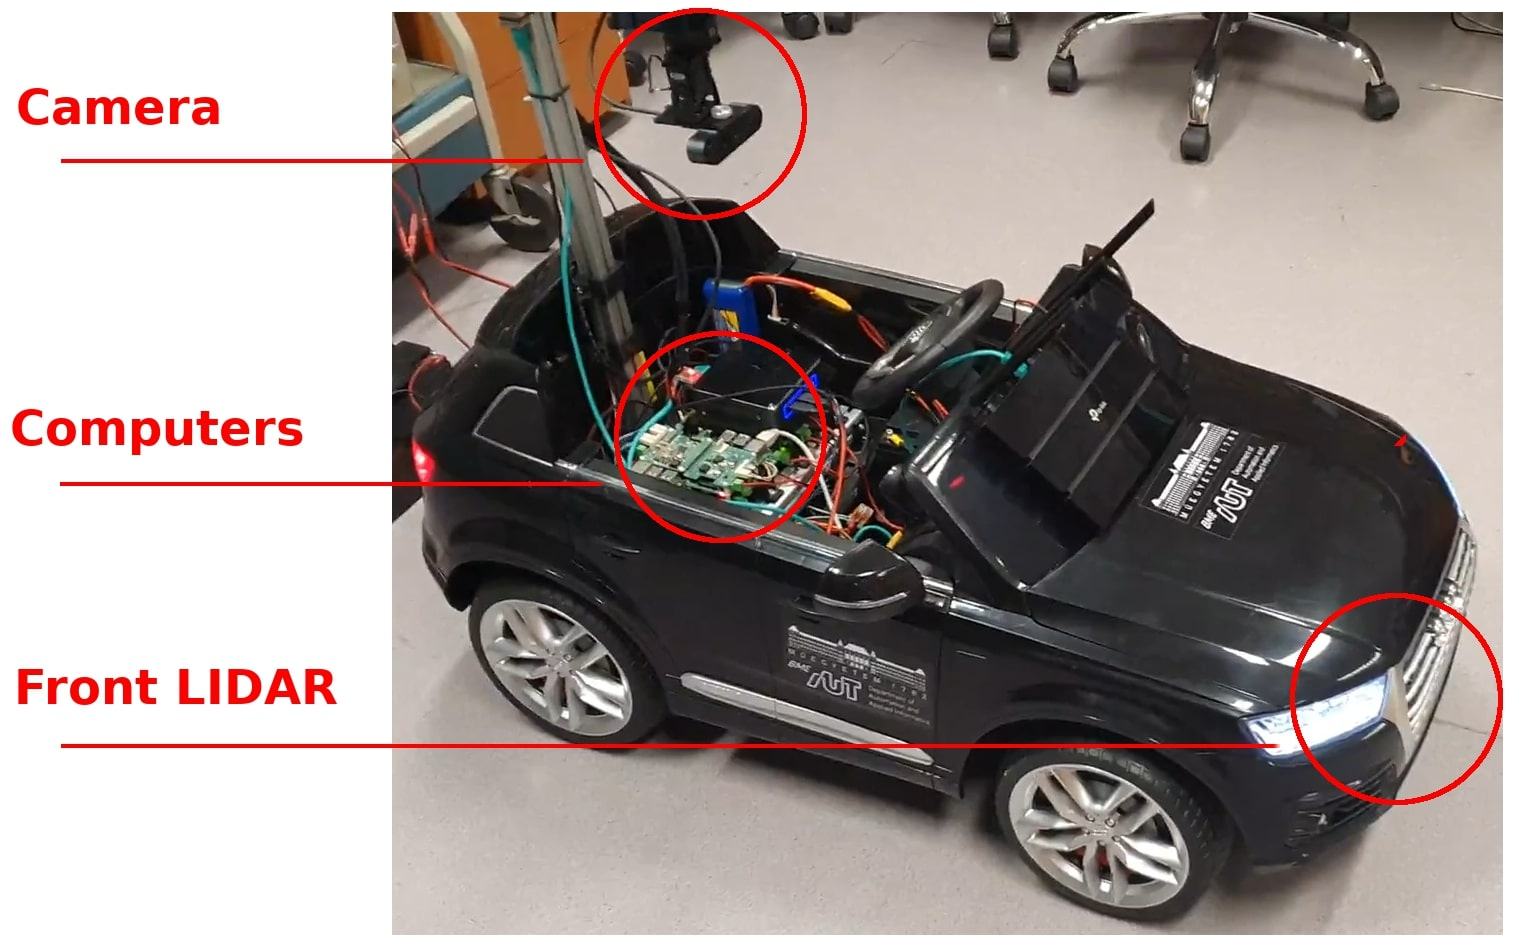
\includegraphics[height=80mm]{figures/raw/car_setup_front.png}
    \caption{The car setup (front side)}
    \label{car_setup_front}
\end{figure}

Amongst others, the car is equipped with a front, a rear and a top LIDAR, a camera, inertial sensors, ultrasonic distance sensors, several Raspberry Pi-s and an Intel NUC computer.

\begin{figure}[!ht]
    \centering
    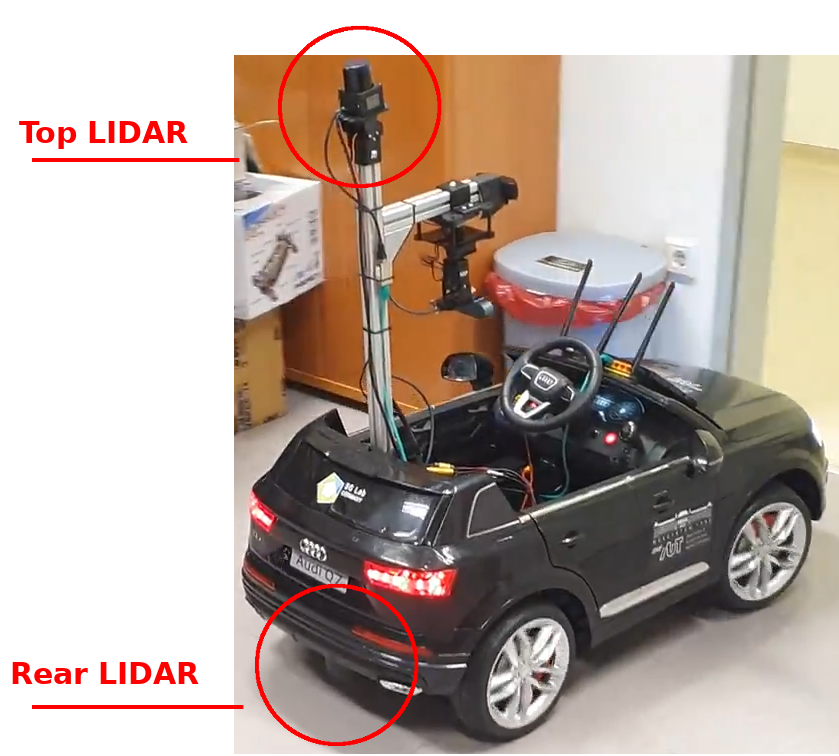
\includegraphics[height=100mm]{figures/raw/car_setup_rear.png}
    \caption{The car setup (rear side)}
    \label{car_setup_rear}
\end{figure}

The vehicle supports the development and testing of multiple smaller projects (mapping and navigation algorithms, control modules, etc.), all contributing to the car becoming more and more able to drive itself. For these sub-projects, the above mentioned sensors are all needed, later I will explain them in detail. These sensors and computers provide a good hardware base for the project, but they are not all that's necessary. A project of this complexity cannot be maintained without a reliable and robust software framework to build upon. This framework is ROS.

\subsection{About ROS}

\begin{quote}
The Robot Operating System (ROS) is a \textbf{set of software libraries} and tools that help you build robot applications. From drivers to state-of-the-art algorithms, and with powerful developer tools, ROS has what you need for your next robotics project. And it's all \textbf{open source}.
\end{quote}

The above description is quoted\footnote{As the short descriptions on ROS pages are pretty straightforward, I am going to quote from them whenever possible.} from their \href{https://www.ros.org/}{website}. Short as it may be, their description does point out that ROS is a software framework for robotic applications. Wikipedia also has a brief and comprehensible \href{https://en.wikipedia.org/wiki/Robot_Operating_System}{article} about ROS, in which it states that:

\begin{quote}
Although ROS is \textbf{not an operating system}, it provides services designed for a heterogeneous computer cluster such as hardware abstraction, low-level device control, implementation of commonly used functionality, message-passing between processes, and package management. Running sets of ROS-based processes are represented in a \textbf{graph architecture} where processing takes place in nodes that may receive, post and multiplex sensor data, control, state, planning, actuator, and other messages. Despite the importance of reactivity and low latency in robot control, ROS itself is not a real-time OS (RTOS). It is possible, however, to integrate ROS with real-time code.
\end{quote}

So what is ROS exactly? It is a framework that helps building robot applications. It is basically a large set of software components with an own build system. It is not an operating system, therefore it needs one under it. Although it may be installed on Debian and Windows 10 as well, its main target OS is Ubuntu. For this reason, the chosen OS for the computers in the project became Ubuntu (versions Artful and Bionic are supported).

All ROS applications have a graph architecture, meaning that they are considered as a set of separate processes (nodes) that are connected via messages. These message are published on topics, which are message bus names. The standard defines some popular message types, but supports custom messages as well. The communication through messages is based on the publish-subscribe model, a publisher provides some data on a topic in the form of messages that all subscribed nodes can read. The implementation of the message-passing, the used networks layer and the transmission and reception of the messages are hidden from the application. ROS handles the delivery between different processes and even different hosts.

What ROS guarantees is a stable build system and architecture that helps developers create multi-process applications relatively easy, with reliable message-passing over a configurable transport layer (TCP by default). However, these features would not be enough for developers to consider ROS a relevant candidate for a robotic application framework, easy-to-integrate tools and a detailed documentation are also necessary. Fortunately, ROS does include these.

Its documentation is comprehensible and covers most topics that developers may need to look into. Besides that, a large series of tutorials are also available on their website about getting started with ROS and building simple applications, and also about deeper topics that give major insight to the reader about how ROS tools and features can be used effectively. These tutorials usually demonstrate given features using example applications that are also available for installing.

\subsection{Useful ROS tools}
ROS comes with numerous tools that are plug-and-play compatible any applications, due to that fact that ROS apps are just a set of independent nodes - once opened, these tools become nodes in the ROS graph and they can communicate with the other nodes via messages.

Most of these tools enable the developer to monitor the ROS graph, the existing nodes and the connections among them. Let me mention a few of these programs that proved themselves elementary during working with ROS.

The first one is \href{http://wiki.ros.org/rqt_graph}{rqt\_graph}, which is GUI tool for visualizing the ROS graph - the nodes and the message connections among them. Figure \ref{rqt_graph} shows part of the \textit{vr-car} ROS graph represented using rqt\_graph. The nodes are shown in the ellipses, and the arrows among them are the topics, on which the messages are sent.

\begin{figure}[!ht]
	\centering
	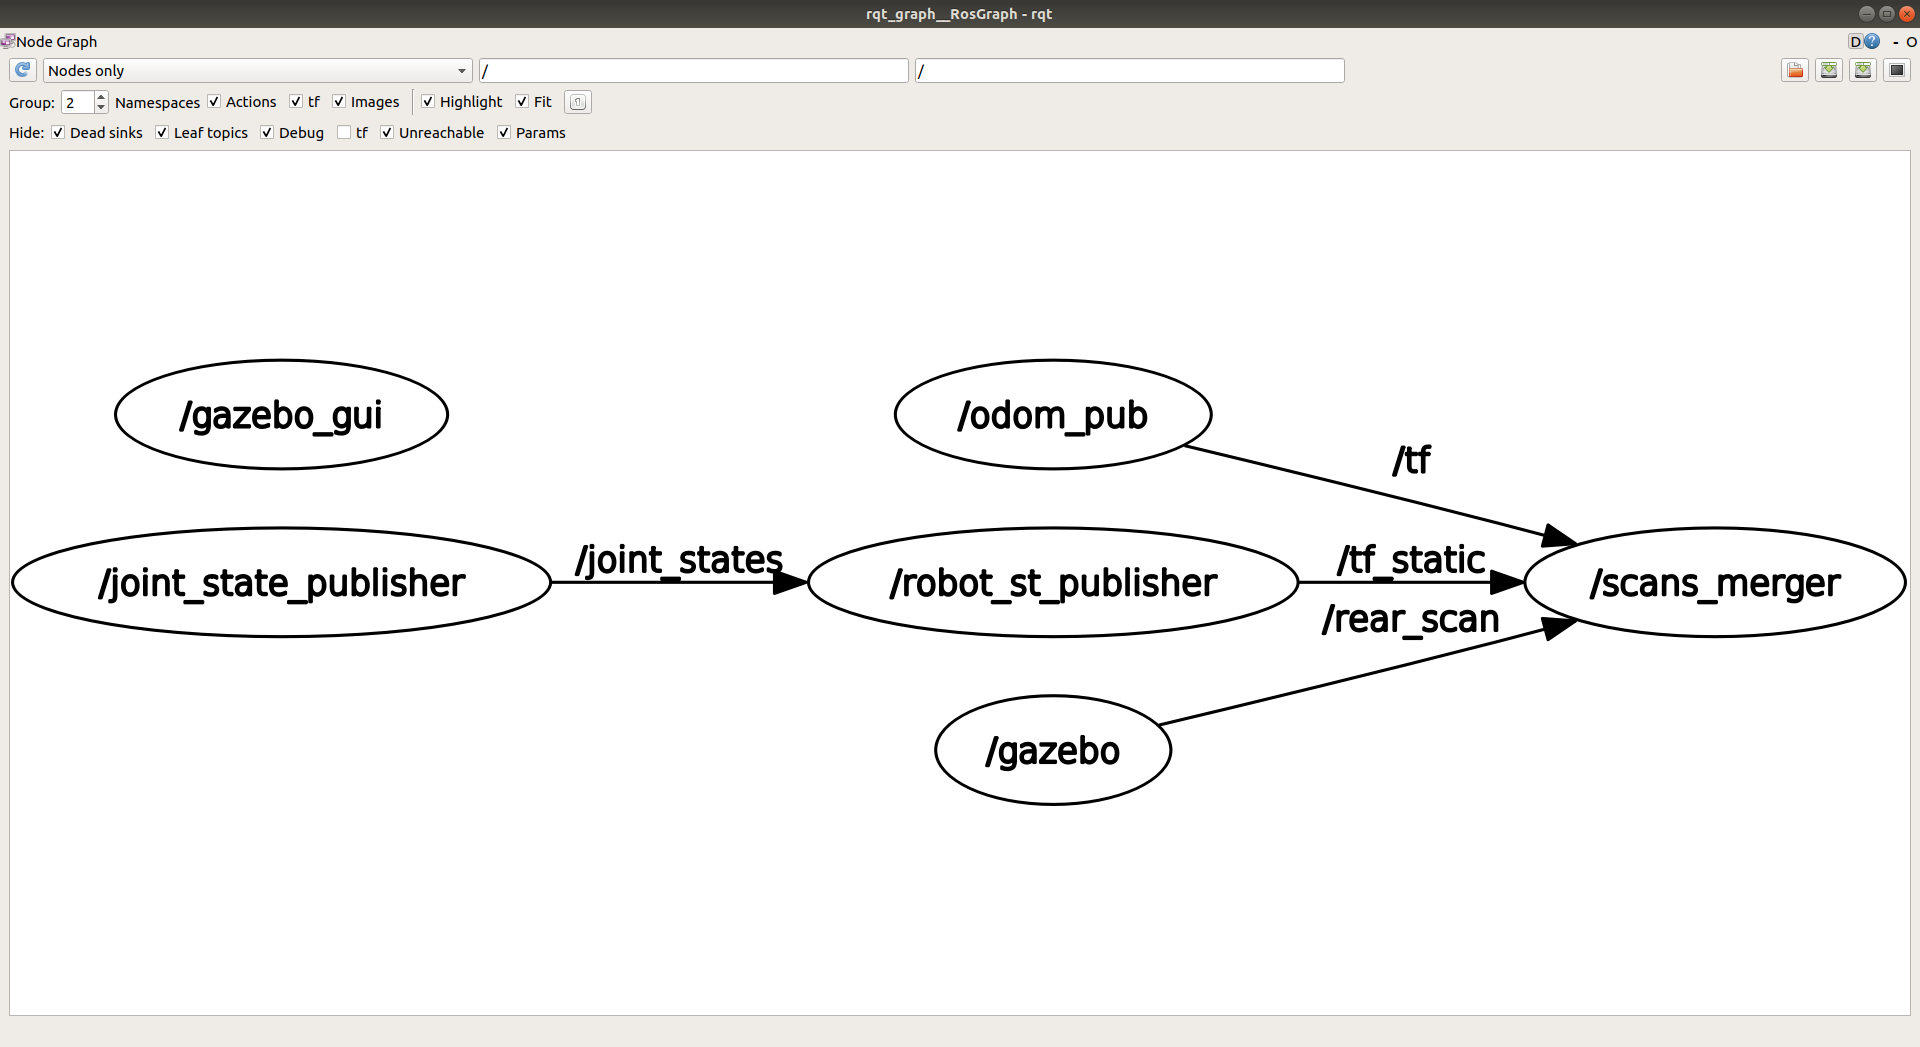
\includegraphics[width=\textwidth]{figures/raw/rqt_graph.png}
	\caption{Visualizing the ROS graph using rqt\_graph}
	\label{rqt_graph}
\end{figure}

A useful command-line tool is \href{http://wiki.ros.org/rostopic}{rostopic}, which may be used to list, search and monitor message topics. For example executing \textit{rostopic list} while the \textit{vr-car} project is running produces the following output:

\begin{minipage}{\textwidth}
\begin{lstlisting}[language=bash]
/Global_planner_wrapper/plan
/camera1/VRcar/camera
/camera1/VRcar/camera/compressed
/camera1/VRcar/camera/compressed/parameter_descriptions
/camera1/VRcar/camera/compressed/parameter_updates
/camera1/VRcar/camera/compressedDepth
/camera1/VRcar/camera/compressedDepth/parameter_descriptions
/camera1/VRcar/camera/compressedDepth/parameter_updates
/camera1/VRcar/camera/theora
/camera1/VRcar/camera/theora/parameter_descriptions
/camera1/VRcar/camera/theora/parameter_updates
/camera1/camera_info
/camera1/parameter_descriptions
/camera1/parameter_updates
/clicked_point
/clock
/front_scan
/gazebo/link_states
/gazebo/model_states
/gazebo/parameter_descriptions
/gazebo/parameter_updates
/gazebo/set_link_state
/gazebo/set_model_state
/initialpose
/joint_states
/lidar_pcl
/lidar_scan
/move_base/global_costmap/costmap
/move_base/global_costmap/costmap_updates
/move_base/local_costmap/costmap
/move_base/local_costmap/costmap_updates
/move_base_simple/goal
/odom
/particlecloud
/path_planner/path_visualization
/path_planner/path_visualization_array
/rear_scan
/rosout
/rosout_agg
/static_grid_updates
/tf
/tf_static
/vrcar/filtered_control
\end{lstlisting}
\end{minipage}

For robotic applications, coordinate transformations and frame tracking in time are essential. Fortunately, ROS has an off-the-shelf solution for coordinate frame handling, this program is called tf. Its \href{http://wiki.ros.org/tf}{documentation} briefly explains that

\begin{quote}
	tf is a package that lets the user keep track of multiple coordinate frames over time. tf maintains the relationship between coordinate frames in a tree structure buffered in time, and lets the user transform points, vectors, etc between any two coordinate frames at any desired point in time.
\end{quote}

And for visualizing the tf tree, \href{http://wiki.ros.org/rqt}{rqt} may be used.

\begin{figure}[!ht]
	\centering
	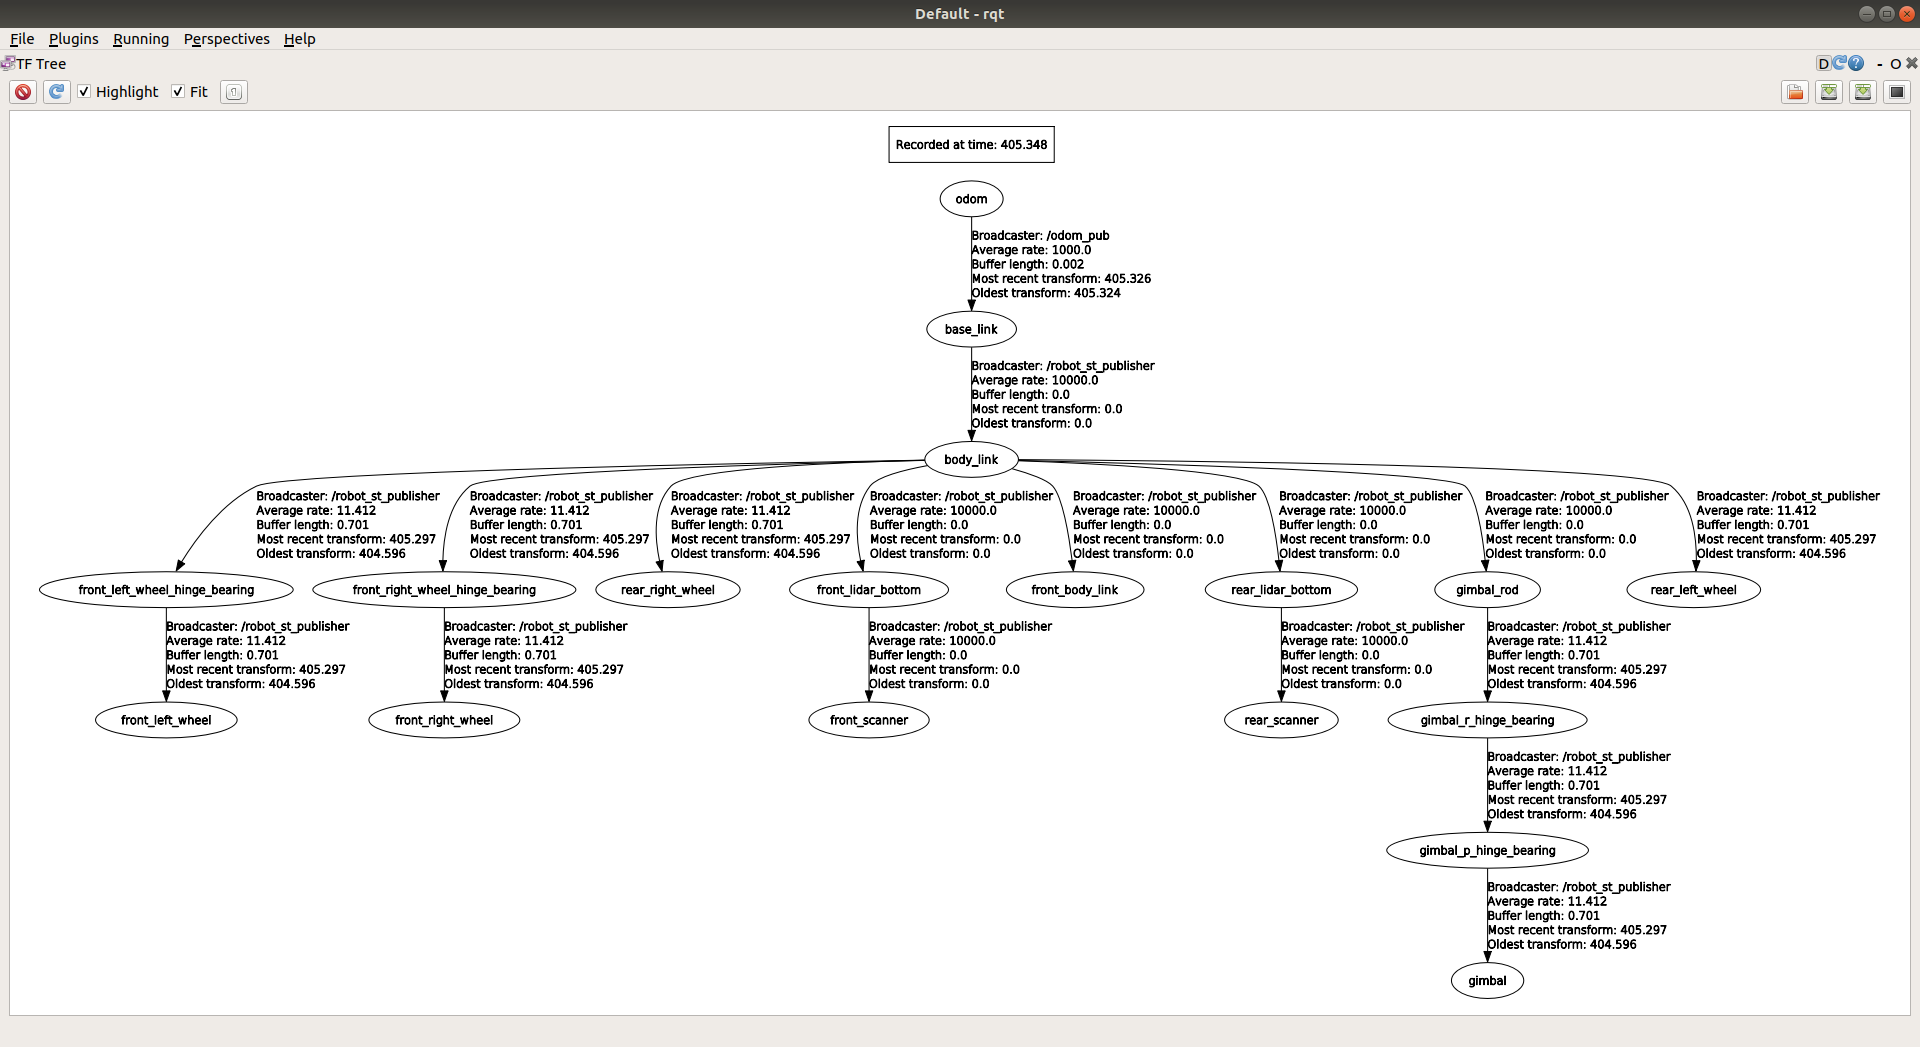
\includegraphics[width=\textwidth]{figures/raw/rqt.png}
	\caption{Visualizing the tf tree using rqt}
	\label{rqt_graph}
\end{figure}

In many cases, algorithm testing consists of various iterations, and it is handy to provide the program the same inputs over and over. For this purpose, ROS has a tool called \href{http://wiki.ros.org/rosbag}{rosbag}, which is able to record and play back messages. This way, the whole ROS graph may be simulated by replaying the node outputs. Debugging algorithms is much easier using rosbag recordings, than having to recreate the same situations running the actual nodes.

The tools mentioned above were programs that help developers to monitor or interfere with the ROS graph and node communications. However, there are standalone applications, too, that are, in a way, independent from the ROS graph overall, they work like regular graph nodes that have certain inputs and outputs.

One of most essential standalone program is \href{http://wiki.ros.org/rviz}{rviz}, a 3D visualization tool. rviz supports a wide range of elements that it can display (camera images, maps, markers, point clouds, robot models, etc.), and the developers also have the option to implement custom display plugins for their own types.

\begin{figure}[!ht]
	\centering
	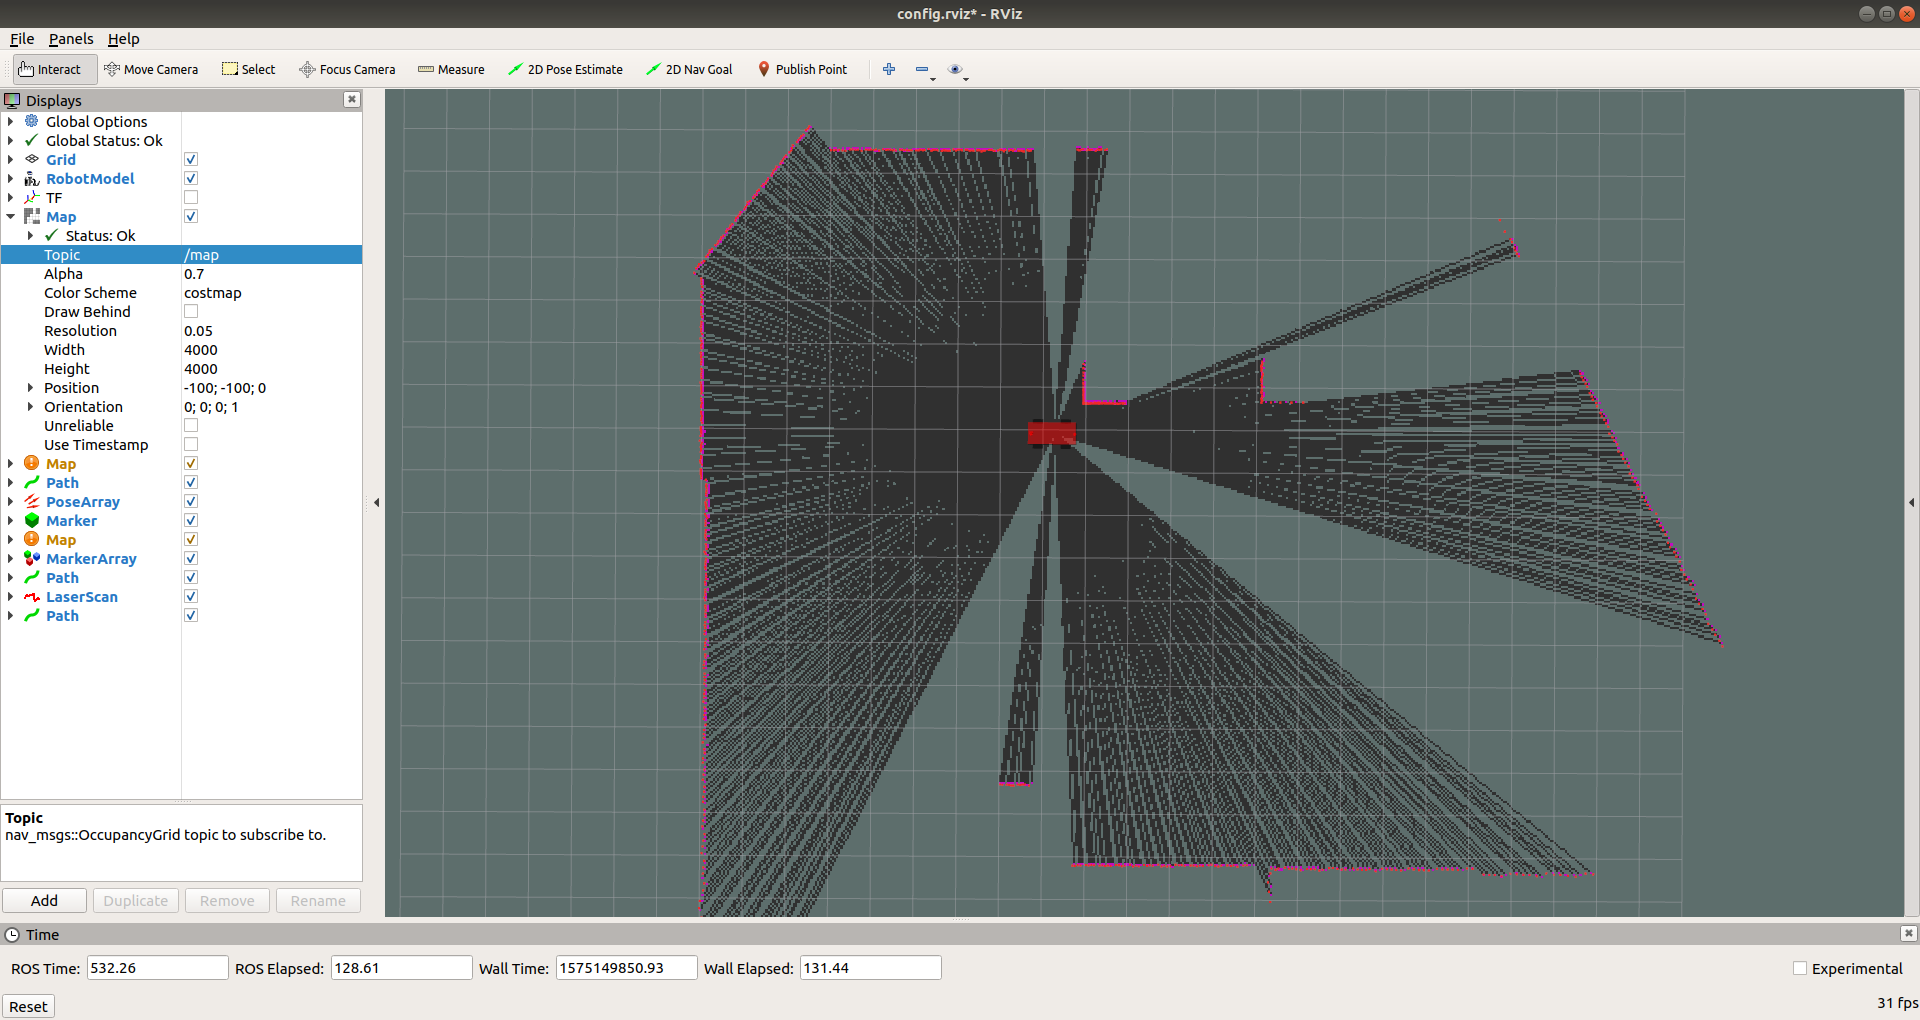
\includegraphics[width=\textwidth]{figures/raw/rviz.png}
	\caption{rviz}
	\label{rviz}
\end{figure}

For vehicle applications such as the \textit{vr-car} project, the typical displayed types are robot models, odometry, trajectories and maps. Just imagining the simplest car driving project we can, displaying the car's position and orientation could be quite useful. Unsurprisingly, rviz supports the visualization of vehicle odometry (see \href{http://wiki.ros.org/rviz/DisplayTypes/Odometry}{Odometry display type}), and according to its documentation:

\begin{quote}
	The Odometry display accumulates a \href{http://docs.ros.org/api/nav_msgs/html/msg/Odometry.html}{nav\_msgs/Odometry} message over time, showing them as arrows.
\end{quote}

So one of the nodes in the project's graph needs to publish the odometry messages, and no further coding is needed, rviz may be opened and odometry will be displayed.

Testing in real life, with the real target host may be difficult and expensive. My diploma project is a perfect example for this, because the test car that operates as the host for the ROS nodes was very rarely accessible for me, as I was developing the project from home. Therefore, having to test my algorithm with the actual \textit{vr-car} vehicle would have been a struggle. Fortunately, \href{http://gazebosim.org/}{Gazebo}, which is an open-source 3D robotics simulator, can be connected to ROS easily. With the help of this software, I was able to simulate the car (alongside the sensors and actuator fixed on it) on my computer. What Gazebo provides according to their website is

\begin{quote}
a robust physics engine, high-quality graphics, and convenient programmatic and graphical interfaces.
\end{quote}

Simulating in Gazebo is relatively more difficult than visualizing in rviz. At every simulation start, Gazebo needs to be given a world describing the simulation environment, and objects to place in the world (e.g. in the simulation represented in figure \ref{gazebo} the world consists of the boxes, while the object placed in the world is the red car).

\begin{figure}[!ht]
	\centering
	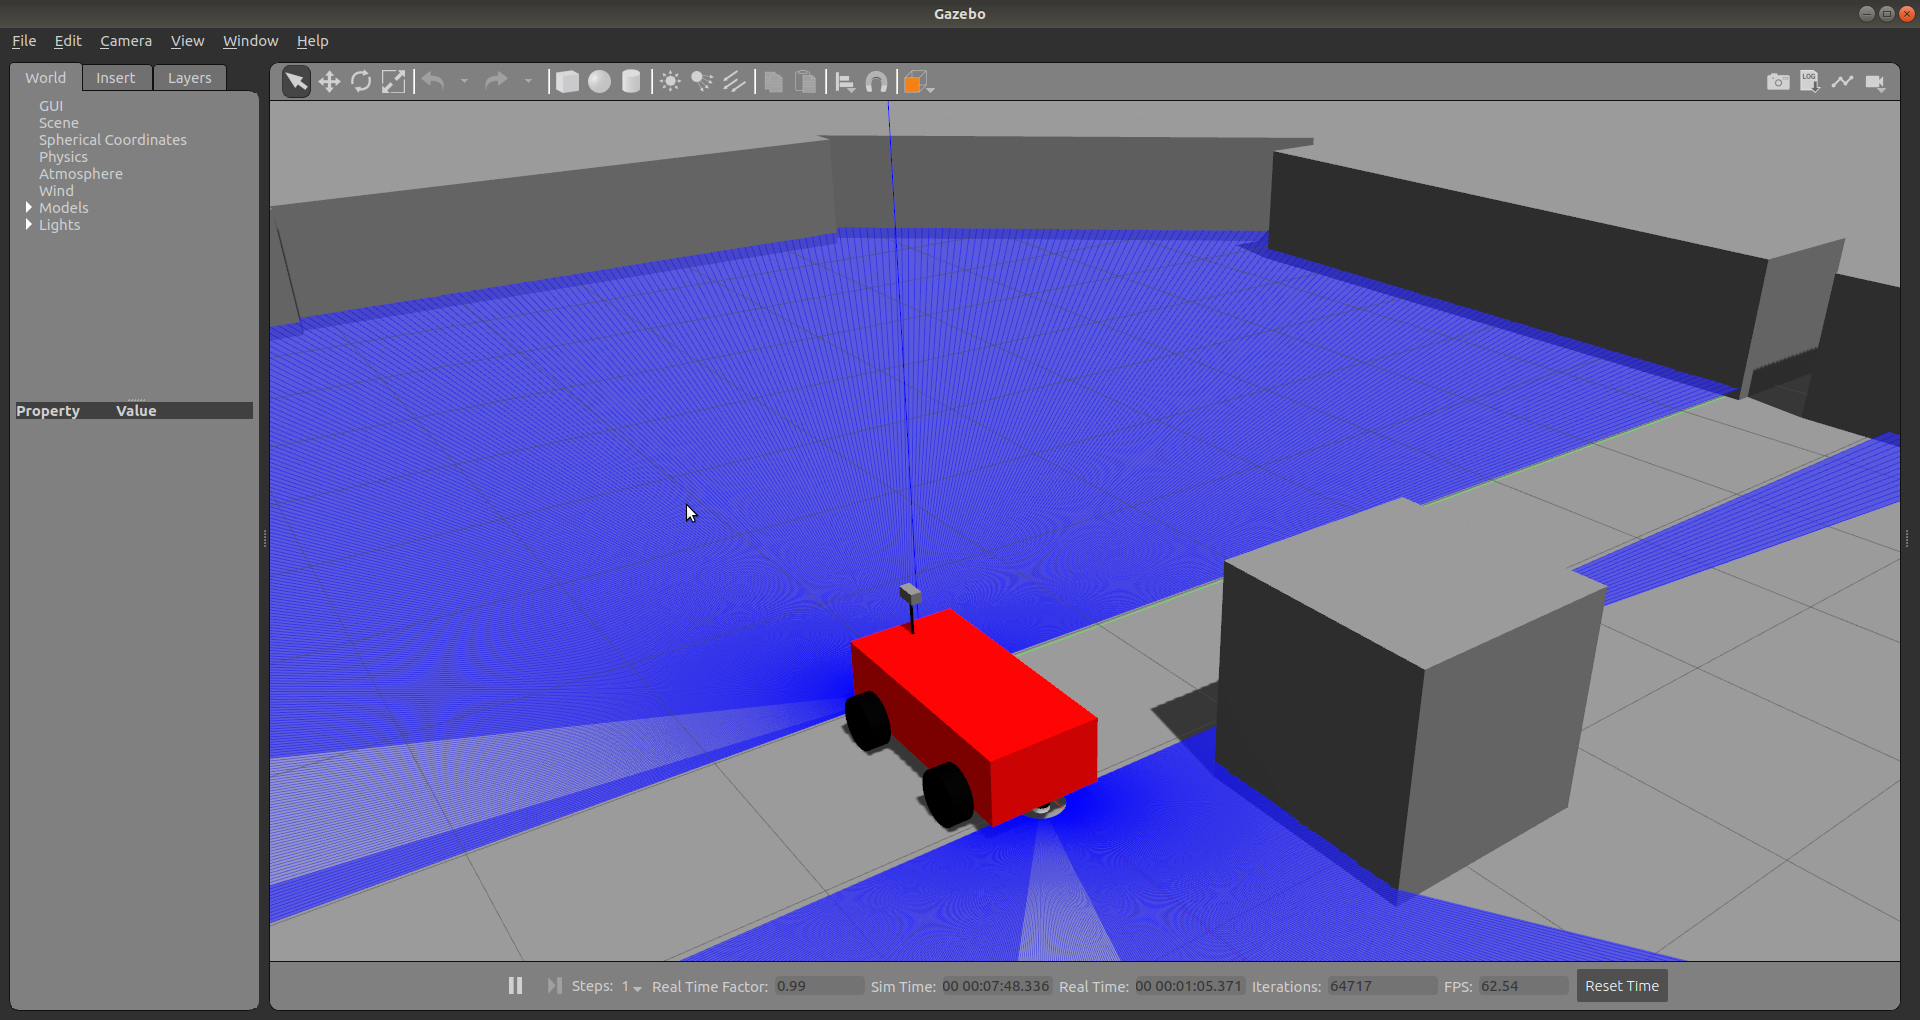
\includegraphics[width=\textwidth]{figures/raw/gazebo.png}
	\caption{Gazebo}
	\label{gazebo}
\end{figure}

The simulated world is defined by an SDF file. Quoting from their\href{http://sdformat.org}{website}:

\begin{quote}
SDF is an XML format that describes objects and environments for robot simulators, visualization, and control. Originally developed as part of the Gazebo robot simulator, SDF was designed with scientific robot applications in mind. Over the years, SDF has become a stable, robust, and extensible format capable of describing all aspects of robots, static and dynamic objects, lighting, terrain, and even physics.
\end{quote}

And the objects are defined by Unified Robot Description Format (URDF) files. These are also XML descriptors that define the structure of an object by links and joints. A basic URDF file containing a single cylinder looks like the following (the example is taken from one of the \href{http://wiki.ros.org/urdf/Tutorials}{URDF tutorials} provided by ROS):

\begin{minipage}{\textwidth}
\begin{lstlisting}[language=XML]
<?xml version="1.0"?>
<robot name="mokifej_foni">
  <link name="base_link">
    <visual>
      <geometry>
        <cylinder length="0.6" radius="0.2"/>
      </geometry>
    </visual>
  </link>
</robot>
\end{lstlisting}
\end{minipage}

Both the SDF world and the URDF models can be opened, edited and saved in Gazebo, thus making the creation and update of these files easy. These models were already created by another member of the \textit{vr-car} project, so I was able to simulate the car without any difficulty or extra work, which was a great help during the development of my algorithms.

In the next sections I am going to explain the ROS graph and the message-passing between nodes using a simplified model of the \textit{vr-car} project, while also describing the features of the application.

\subsection{Remote drive}
The first (and probably simplest to comprehend) feature of the car is the ability to control it remotely, using either a PC keyboard, a joystick or a set of racing wheel and pedals.

In order to make this possible, the car definitely needed a node that controls the car's actuators according to an input actuation. For simplicity, let's assume that this input actuation (a ROS message) contains a target speed and wheel angle that the module has to handle as a reference. Having direct control of the car's motors (the accelerator DC motor and the steering servo) and of the necessary sensors (e.g. a rotary encoder for measuring speed) the control is manageable.

Besides this control module, the graph contains another node, that reads driver interactions (key strokes, joystick state or steering wheel and pedal positions), converts these to driver commands (target actuations) and publishes the correspondent messages that the control node listens to. Note, that these input nodes are implemented separately for the input types - there is a module for keyboard input, one for handling the joystick and a third one for reading the racing wheel and pedal data\footnote{The racing wheel and the throttle and brake pedals are actually handled on a separate Windows host, and their positions are forwarded to another host running ROS.}.

With one input module being active, the graph now contains two processes - the input and the control nodes. These two nodes are communicating through a message that contains speed and wheel angle reference values.

\subsection{\textit{vr-drive}}
Another feature of the car is that the user drive it using one of the input methods listed above while 'seeing what the car sees'. This is implemented by reading the video stream from the camera fixed on the vehicle and transferring it to the user's PC. The user can see the images via an Oculus Rift VR headset. To make it more realistic, the camera on the car is moved in a way that it follows the user's head movements.

\subsection{2D mapping}
As figures \ref{car_setup_front} and \ref{car_setup_rear} show, the car is equipped with a front and a rear 2-dimensional, 360 degree LIDAR. The sensors are hard to see because they are fixed under the chassis. The reason for them being hidden is that they are meant to detect low-height objects as well, therefore they could not have been placed on the top of the car, which would be the usual placement of LIDARs. But as the front LIDAR cannot see backward effectively because it is covered by the wheels (and the same goes for the rear LIDAR looking forward), both LIDARs are needed in order to have a 360 degree view angle. But because the two LIDARs are placed on two different locations on the car, creating one map from their measured values is not trivial. To solve this issue, a special node called \textit{scans\_merger} has been added to project, with the task to merge the scan data from the front and rear LIDARs, thus creating a joined scan.

This scan needs to be evaluated and and kept track over time, while the car is moving, in order to create a map from them. This algorithm could have been initialized as part of the project, but a popular ROS package, \href{http://wiki.ros.org/gmapping}{gmapping} is able to do that outstandingly\footnote{The advantages and drawbacks of gmapping will be discussed in section \ref{chap:mapping}.}.

\subsection{3D mapping}

\begin{figure}[!ht]
	\centering
	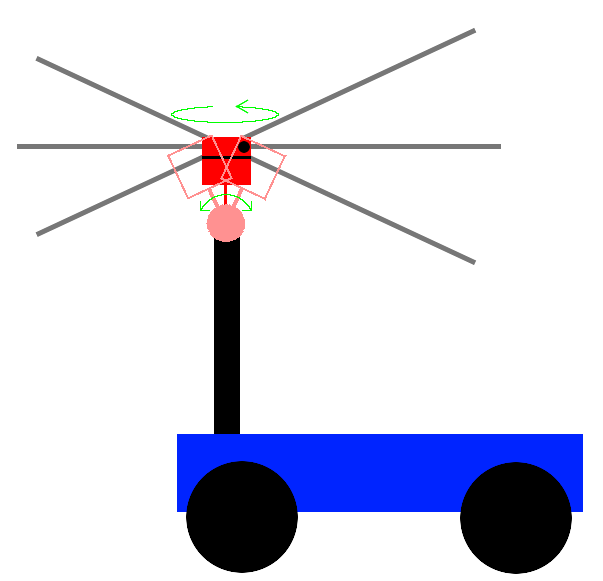
\includegraphics[height=72mm]{figures/raw/3D_lidar.png}
	\caption{Creating a 3D map by tilting a 2D LIDAR}
	\label{tilt_lidar}
\end{figure}

3D mapping is implemented using the front LIDAR, which is also a 2-dimensional, 360 degree sensor, but it is placed on a gimbal, and is tilted forward and backward with ~0.5 Hz frequency. Because of the tilting movement, the LIDAR scans a different plane in every step. And merging these planes creates a 3D map (see figure \ref{tilt_lidar}).

\subsection{Navigation}
The project has a goal to make the car able to navigate from its actual position to a desired target position in the map. In order to do that, it needs a reliable map of its environment. As I mentioned earlier, gmapping produces a good-quality map, therefore the navigation algorithm uses that as its base. Looking at the navigation node as a black box (other members of the project have implemented and are still working on it, its internal logic is not relevant for my diploma project), it receives a destination point in a ROS message, and produces a path in another. Both the input and output messages are standard ROS messages that I will explain in detail later. For providing the destination point for the algorithm, there exists several possibilities, but one of the most straightforward method is through rviz. The visualization tool is not only capable of displaying content, but it has a feature that the user can select a '2D Nav Goal' in the view, and the selected point will be sent out on a specific topic into the graph. A very effective and elegant way is to combine the map drawing with this feature for creating an interface that enables the user to decide where the next destination point should be, by clicking somewhere in the map. Needless to say, giving a target position for the navigation node is implemented using this method.

\tikzset{
	base_node/.style    = {rectangle, rounded corners, draw=black,
		minimum width=4.5cm, minimum height=1cm,
		text centered, font=\sffamily},
	inout_node/.style   = {base_node, fill=blue!30},
	vr_car_node/.style  = {base_node, fill=orange!15},
	decoration={brace},
	tuborg/.style={decorate},
	tubnode_left/.style={midway, left=2pt},
	tubnode_right/.style={midway, right=2pt}
}

\begin{figure}[!ht]
	\begin{tikzpicture}[
	node distance=1.5cm,
	every node/.style={fill=white, font=\sffamily}, align=center]
	% Input nodes
	\node (front_scan)       [inout_node]                                      {Front scan};
	\node (rear_scan)        [inout_node, xshift=5.0cm]                        {Rear scan};
	\node (top_scan)         [inout_node, xshift=10.0cm]                       {Top scan};
	\node (control_input)    [inout_node, xshift=7.5cm, yshift=-6.0cm]         {Control input (joystick)};
	% Active nodes
	\node (scans_merger)     [vr_car_node, below of=rear_scan]                 {Scans merger};
	\node (gmapping)         [vr_car_node, below of=scans_merger]              {gmapping};
	\node (navigation)       [vr_car_node, below of=gmapping]                  {Navigation};
	\node (3d_mapping)       [vr_car_node, below of=top_scan]                  {3D mapping};
	\node (control)          [vr_car_node, below of=navigation, yshift=-1.5cm] {Control};
	% Output node
	\node (actuators)        [inout_node, below of=control]                    {Actuators};
	% Connections
	\draw[->]     (front_scan) -- (scans_merger);
	\draw[->]      (rear_scan) -- (scans_merger);
	\draw[->]   (scans_merger) -- (gmapping);
	\draw[->]       (gmapping) -- (navigation);
	\draw[->]  (control_input) -- (control);
	\draw[->]     (navigation) -- (control);
	\draw[->]        (control) -- (actuators);
	\draw[->]       (top_scan) -- (3d_mapping);
	\end{tikzpicture}
	\caption{The original \textit{vr-car} graph}
	\label{original_vr_car_graph}
\end{figure}

Now that the main features of the \textit{vr-car} has been listed and briefly explained, let me introduce what my part of the project was, and how it fits into the existing graph. So far, the graph consists of the nodes represented in figure \ref{original_vr_car_graph}. Note, that this image is a simplified version of the actual \textit{vr-car} graph, it does not contain all the existing nodes, and some nodes have been merged into one for the sake of simplicity.

\subsection{Avoiding moving obstacles}
My task as a diploma project was to design, implement and tune two nodes, that embed themselves into the existing graph.

The first one is a mapping node. While there are numerous mapping implementations available in ROS (see gmapping for one example), none of them handles moving objects correctly (I am providing a detailed reasoning in section \ref{chap:mapping}). So the goal of the mapping node was to separate the static points from the moving objects in the map.

The other node was a local trajectory planner node, that (based on the mapping nodes output of static and dynamic objects) performs local obstacle avoidance considering not only the position but also the velocities of the surrounding obstacles.

\tikzset{
	base_node/.style    = {rectangle, rounded corners, draw=black,
		minimum width=4.5cm, minimum height=1cm,
		text centered, font=\sffamily},
	inout_node/.style   = {base_node, fill=blue!30},
	common_node/.style  = {base_node, fill=orange!15},
	dynamic_node/.style = {base_node, fill=green!30},
	static_node/.style  = {base_node, fill=red!30},
	decoration={brace},
	tuborg/.style={decorate},
	tubnode_left/.style={midway, left=2pt},
	tubnode_right/.style={midway, right=2pt}
}

\tikzset{
	base_node/.style    = {rectangle, rounded corners, draw=black,
		minimum width=4.5cm, minimum height=1cm,
		text centered, font=\sffamily},
	inout_node/.style   = {base_node, fill=blue!30},
	vr_car_node/.style  = {base_node, fill=orange!15},
	added_node/.style   = {base_node, fill=green!30},
	decoration={brace},
	tuborg/.style={decorate},
	tubnode_left/.style={midway, left=2pt},
	tubnode_right/.style={midway, right=2pt}
}

\begin{figure}[!ht]
	\begin{tikzpicture}[
	node distance=1.5cm,
	every node/.style={fill=white, font=\sffamily}, align=center]
	% Input nodes
	\node (front_scan)       [inout_node]                                                {Front scan};
	\node (rear_scan)        [inout_node, xshift=5.0cm]                                  {Rear scan};
	\node (top_scan)         [inout_node, xshift=10.0cm]                                 {Top scan};
	\node (control_input)    [inout_node, xshift=7.5cm, yshift=-6.0cm]                   {Control input (joystick)};
	% Active nodes
	\node (scans_merger)     [vr_car_node, below of=rear_scan]                           {Scans merger};
	\node (gmapping)         [vr_car_node, below of=scans_merger]                        {gmapping};
	\node (navigation)       [vr_car_node, below of=gmapping]                            {Navigation};
	\node (3d_mapping)       [vr_car_node, below of=top_scan]                            {3D mapping};
	\node (control)          [vr_car_node, below of=navigation, yshift=-3.0cm] 			 {Control};
	% Added nodes
	\node (mapping)          [added_node, below of=front_scan]                           {Mapping};
	\node (local_planner)    [added_node, below of=mapping, xshift=2.5cm, yshift=-4.5cm] {Local planner};
	% Output node
	\node (actuators)        [inout_node, below of=control]                              {Actuators};
	% Connections
	\draw[->]     (front_scan) -- (scans_merger);
	\draw[->]      (rear_scan) -- (scans_merger);
	\draw[->]   (scans_merger) -- (gmapping);
	\draw[->]       (gmapping) -- (navigation);
	\draw[->]  (control_input) -- (control);
	\draw[->]        (control) -- (actuators);
	\draw[->]       (top_scan) -- (3d_mapping);
	% Added connections
	\draw[->]     (front_scan) -- (mapping);
	\draw[->]      (rear_scan) -- (mapping);
	\draw[->]        (mapping) -- (local_planner);
	\draw[->]  (control_input) -- (local_planner);
	\draw[->]     (navigation) -- (local_planner);
	\draw[->]  (local_planner) -- (control);
	\end{tikzpicture}
	\caption{The modified \textit{vr-car} graph}
	\label{modified_vr_car_graph}
\end{figure}

The \textit{vr-car} graph with the two additional nodes is represented in figure \ref{modified_vr_car_graph}. The mapping nodes uses the raw front and rear LIDAR scans as its inputs for the map creation. The local trajectory planner node cuts the connection between the Navigation and the Control nodes, because it overrides the pre-calculated path based on the static and dynamic obstacles in the car's environment.
\include{content/hardware}
\chapter{Mapping}

\section{Method}
This chapter decribes the process of building a separate static and a dynamic map (containing non-moving and moving obstacles, respectively) based on radial distance measurements (in this case provided by a LIDAR). Isolating the static and the moving obstacles from each other has its difficulties but also its advantages. First of all, the implemented local track planner calculates safer, more optimized paths if it is informed of both the static and the dynamic obstacles along the path. Secondly, \href{https://en.wikipedia.org/wiki/Simultaneous_localization_and_mapping}{SLAM} (Simultaneous localization and mapping) algorithms work better if the their input contains only static objects in the space, because they build an internal map of the world. Passing detections of moving obstacles to a SLAM algorithm may lead to worse localization quality, as they may ruin this map.

As a first subtask of the mapping project, I checked if any implementation is avaiable already, that can handle dynamic objects. The only possible candidate was \href{http://wiki.ros.org/gmapping}{gmapping}, which is a popular ROS package, used in a wide variety of applications that require map-building and localization. Its SLAM algorithm takes LIDAR measurements as its input and generates an occupancy grid (a 2D map) of the car's environment. By using this map it is able to make corrections to the car's odometry-based position and orientation, which is usually inaccurate. I tried out the package, and the result maps were promising, the generated map was insensitive to the car's longitudinal movements and its rotations. But unfortunately, gmapping's SLAM does not support dynamic objects. See \autoref{chap:static_map} for further details. Therefore, gmapping could not be used as the producer of the static map. But that didn't mean it couln't be used for its second feature, localization. Note, that the mapping implementation I made is not a SLAM algorithm, it is not able to make corrections to the car's pose. So for that purpose, I still needed the help of gmapping, which proved to be very reliable at localization. But the static map-building needed to be implemented internally.

In order to create two disjunct maps, one static and one dynamic, the key element of the process is the separation of the moving and non-moving obstacles of the measured points. After determining these two disjunct set of points, the maps can be converted to any desired or required format. Static maps are usually published as occupancy grids, while dynamic obstacles need to present information about their speed vector. Occupancy grids do not group the grid points according to their probabilities, therefore they do not know about the obstacles' borders and areas\footnote{In this project, 2D LIDARs were used, therefore the measured objects were seen as 2D shapes that have areas, not 3D objects that have volumes}. Dynamic obstacles however can be either represented as separate points with their own speed vectors, or groups of points, each groups having one speed vector. I chose the latter representation, thus publishing groups that contain a set of points (all the points, ideally) of the same obstacle. This way there is a one-to-one relationship between moving obstacles and groups. The separation and grouping methods of the mapping process is shown on diagram \ref{mapping_method}.

\tikzset{
     base_node/.style = {rectangle, rounded corners, draw=black,
                         minimum width=5cm, minimum height=1cm,
                         text centered, font=\sffamily},
  inout_node/.style   = {base_node, fill=blue!30},
  common_node/.style  = {base_node, fill=orange!15},
  dynamic_node/.style = {base_node, fill=green!30},
  static_node/.style  = {base_node, fill=red!30},
  decoration={brace},
  tuborg/.style={decorate},
  tubnode_left/.style={midway, left=2pt},
  tubnode_right/.style={midway, right=2pt}
}

\begin{figure}[!ht]
    \begin{tikzpicture}[
            node distance=1.5cm,
            every node/.style={fill=white, font=\sffamily}, align=center]
        % Node descriptions
        \node (scan)            [inout_node]                                   {Input scan};
        \node (convert_abs)     [common_node, below of=scan]                   {Convert to absolute points};
        \node (dynamic_points)  [common_node, below of=convert_abs]            {Find dynamic points};
        \node (groups)          [common_node, below of=dynamic_points]         {Make dynamic groups};
        \node (separate)        [common_node, below of=groups]                 {Separate static points from groups};
        % Dynamic nodes
        \node (areas)           [dynamic_node, below of=separate, xshift=-3cm] {Measure areas};
        \node (tracking)        [dynamic_node, below of=areas]                 {Track groups};
        \node (publish_dynamic) [inout_node, below of=tracking]                {Publish dynamic obstacles};
        % Static nodes
        \node (update_map)      [static_node, below of=separate, xshift=3cm]   {Update static map};
        \node (publish_static)  [inout_node, below of=update_map]              {Publish static scan};
        % Connections
        \draw[->]           (scan) -- (convert_abs);
        \draw[->]    (convert_abs) -- (dynamic_points);
        \draw[->] (dynamic_points) -- (groups);
        \draw[->]         (groups) -- (separate);
        % Dynamic connections
        \draw[->]       (separate) -- (areas);
        \draw[->]          (areas) -- (tracking);
        \draw[->]       (tracking) -- (publish_dynamic);
        % Static connections
        \draw[->]       (separate) -- (update_map);
        \draw[->]     (update_map) -- (publish_static);
        % Decorations
        \draw[tuborg, decoration={brace}] let \p1=(scan.north), \p2=(separate.south) in
            ($(\x1+3.4cm, \y1)$) -- ($(\x1+3.4cm, \y2)$) node[tubnode_right] {Separation + grouping};
        \draw[tuborg, decoration={brace}] let \p1=(areas.north), \p2=(publish_dynamic.south) in
            ($(\x1-3cm, \y2)$) -- ($(\x1-3cm, \y1)$) node[tubnode_left] {Dynamic};
        \draw[tuborg, decoration={brace}] let \p1=(update_map.north), \p2=(publish_static.south) in
            ($(\x1+3cm, \y1)$) -- ($(\x1+3cm, \y2)$) node[tubnode_right] {Static};
    \end{tikzpicture}
    \caption{Mapping method}
    \label{mapping_method}
\end{figure}

The diagram consists of 3 subgraphs - these are also marked on the diagram. The first, and most important is the separation and grouping of dynamic points. The second section describes the additional calculations that need to be done for the dynamic obstacles, and consists the documentation for the message structure definining these dynamic obstacles. The third section is about the static map that is built from the static points. The next sections are going to explain these subgraphs in detail.

\section{Separation and grouping}
\label{chap:separation_and_grouping}
This section describes the method of separating dynamic and static points of the input scan. This step is essential in the pipeline of creating two disjunct maps.

\subsection{Input scan}
The input of the mapping algorithm is a 2D LIDAR scan, consisting of radial distance measurements. Two types of LIDARs were used in the project, \href{http://www.slamtec.com/en/lidar/a1}{RPLidar A1} and \href{http://www.slamtec.com/en/lidar/a2}{RPLidar A2}.
Both types have the following specifications:

\begin{center}
    \begin{tabular}{ | c | c | }
        \hline
        Scan rate           & 10 Hz            \\
        \hline
        Sample rate         & 8000 samples/sec \\
        \hline 
        Distance resolution & 0.2 centimeters  \\
        \hline 
        Angular resolution  & 1°               \\
        \hline 
        Detection range     & 12 meters        \\
        \hline
    \end{tabular}
\end{center}

The devices proved to be reliable, and for a project of this volume, their frequencies, resolutions and ranges were adequate. Their output after each measurement sequence is an array of radial distances, that can be visualized easily using rviz.

\begin{figure}[!ht]
    \centering
    \subfloat[Gazebo simulation]
    {
        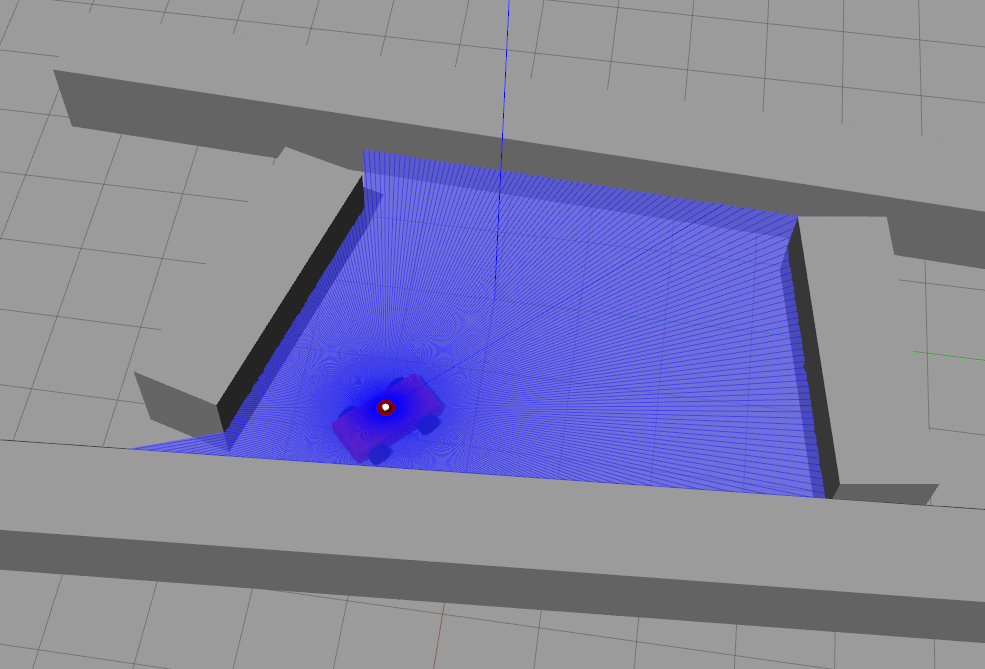
\includegraphics[height=48mm]{figures/raw/gazebo_lidar_scan.png}
        \label{gazebo_lidar_scan}
    }
    \subfloat[rviz visualization]
    {
    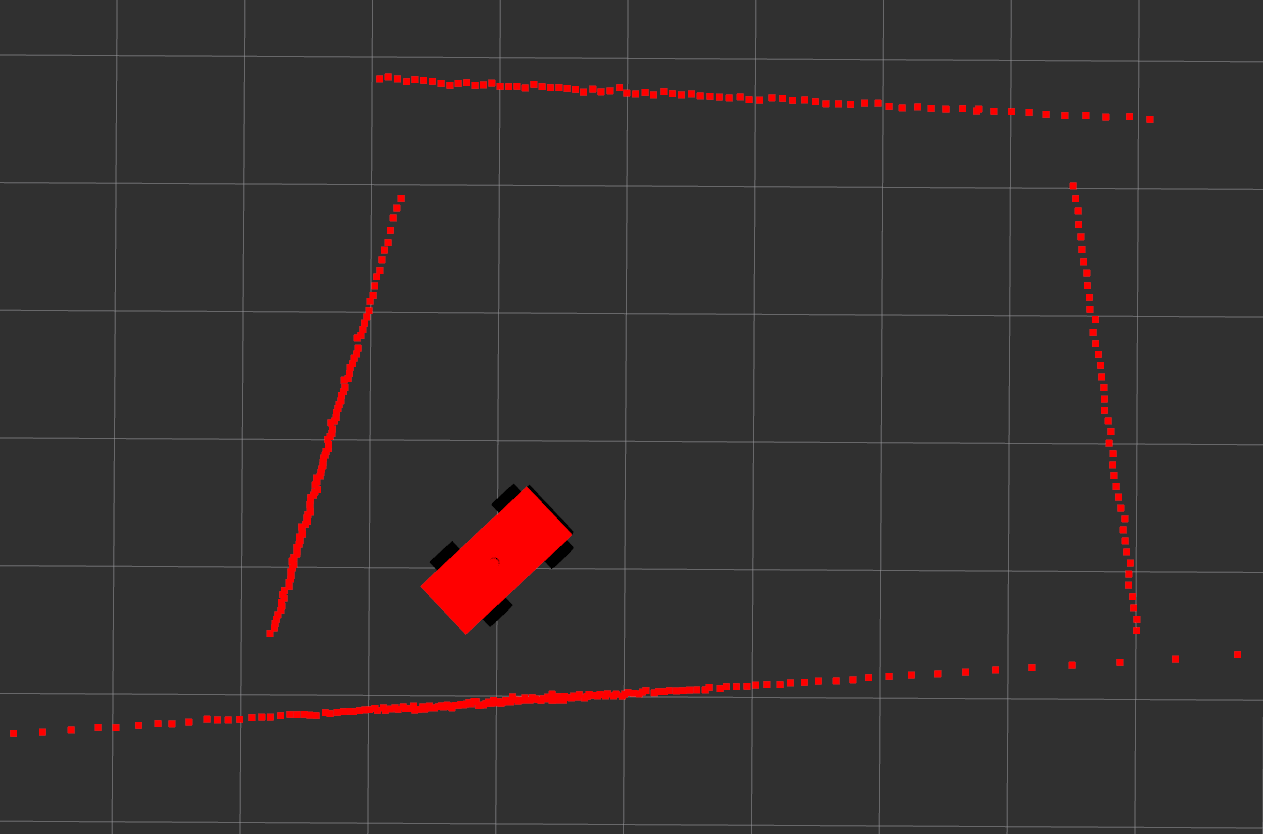
\includegraphics[height=48mm]{figures/raw/rviz_lidar_scan.png}
        \label{rviz_lidar_scan}
    }
    \caption{LIDAR scan}
    \label{lidar_scan}
\end{figure}

\subsection{Absolute points}
For static map-building, absolute points\footnote{Absolute points are not relative to the car, but to a fix base point.} are needed in the space, and static-dynamic point separation also uses absolute points, so firstly, these radial distances need to be transformed. However, the internal static map and the static-dynamic separation use different coordinate systems. In order to understand the need for this, let's take a look at figure \ref{rqt_input}.

\begin{figure}[!ht]
    \centering
    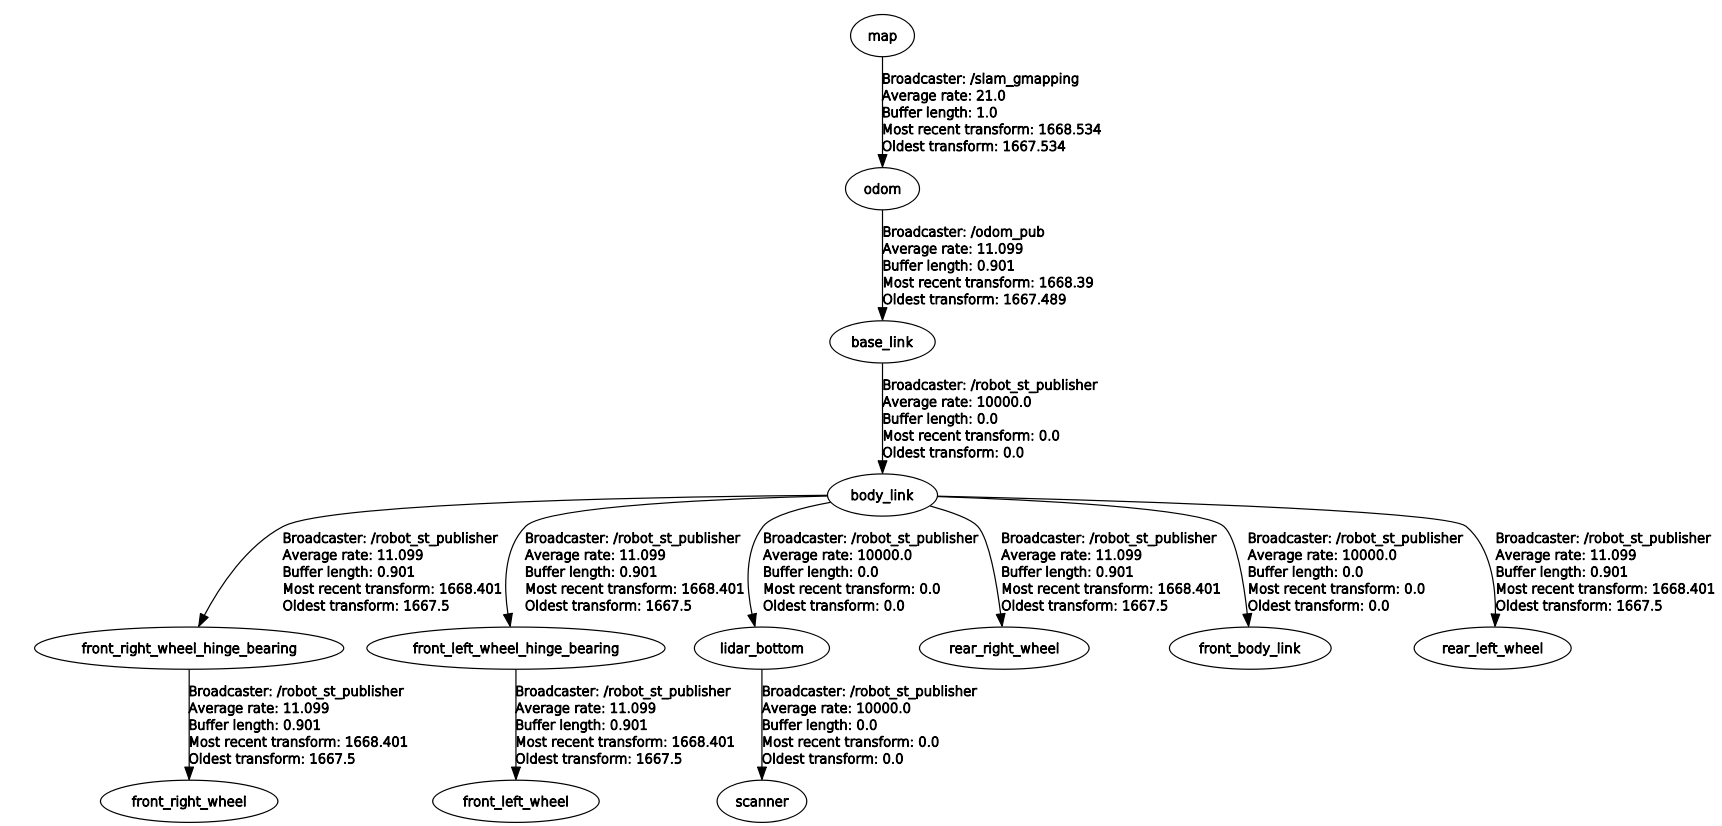
\includegraphics[height=130mm]{figures/raw/rqt_input.png}
    \caption{Coordinate frames}
    \label{rqt_input}
\end{figure}

As the figure shows, there are 3 coordinate frames that are important to the current case. The \textit{odom} frame is the car odometry's coordinate system. It is calculated from values measured on the vehicle, such as servo position and speed. The \textit{scanner} frame is the LIDAR's coordinate system. The transformation between \textit{odom} and \textit{scanner} is basically the pose of the LIDAR, relative to the car. The \textit{map} frame is the output of gmapping's localization. Basically, gmapping takes the car odometry and the LIDAR scans as its input, and corrects the odometry using SLAM. As a result the difference between frames \textit{map} and \textit{odom} will increase with time.

The internal static map in my imlpementation uses this corrected \textit{map} frame as the base for its points, so that its error is minimized. But unfortunately, the static-dynamic separation method cannot use this frame. The reason is that this frame does not get updated on every new scan, but with a much slower frequency. Therefore there are 'jumps' in the \textit{map} frame, which would cause false dynamic point detections (see \autoref{chap:dynamic_points}). To avoid this undesired situation, the static-dynamic separation uses the \textit{odom} frame as its base, which is more continuous than the \textit{map} frame.

Therefore, two transformations are needed for each input point. The transformations are calculated using \href{http://wiki.ros.org/tf}{tf}, which maintains the relationship between coordinate frames in a tree structure (see figure \ref{rqt_input}) buffered in time, and makes the transformation of points, vectors, etc possible at any desired point in time.

\subsection{Dynamic points}
\label{chap:dynamic_points}
The next step is similar to a creating a subtraction image in image processing, where subtracting two images, taken from the same position but at a different time, results in an image that amplifies the movements between the snapshots. Previous methods\cite{RealTimeDynamicObjectDetection} that I studied before starting my implementation are also based on this step. The aim of this algorithm unit is basically the same: selecting the points from the input that are likely to be part of a moving mass. This is done by finding the points among the current measurements that have not been present in the previous ones.

This step is best explainable in practice. Let's assume that the position and orientation of the LIDAR is fix, and one object (e.g. a car) in the detected area is moving. Figure \ref{obstacle_movement} shows this situation. On the image, the pale contour represents the previous pose of the object, and the current state is blue.

\begin{figure}[!ht]
    \centering
    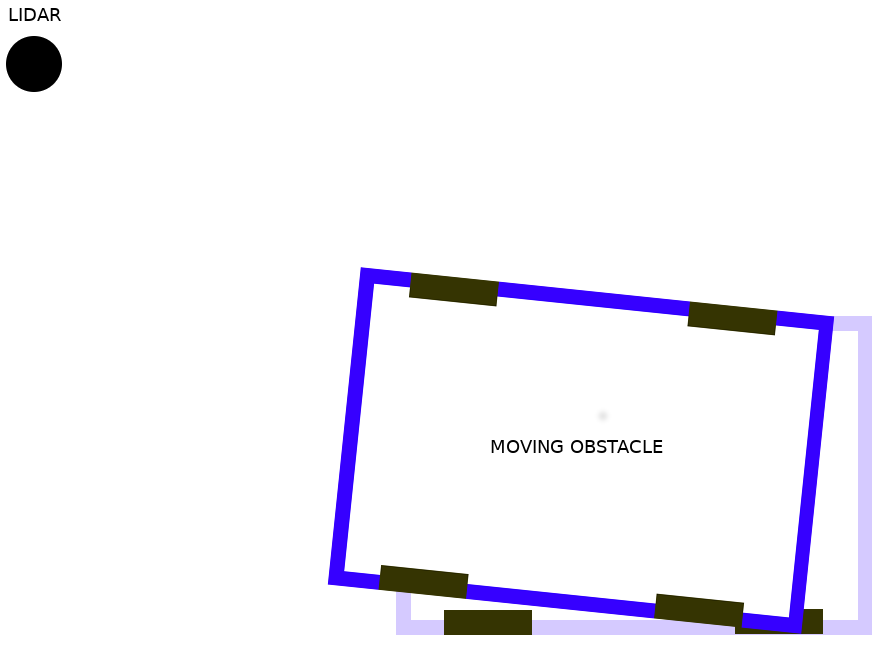
\includegraphics[height=80mm]{figures/raw/obstacle_movement.png}
    \caption{The obstacle is moving}
    \label{obstacle_movement}
\end{figure}

Figure \ref{obstacle_movement_lidar} shows how the LIDAR detects the moving object in two different timesnaps. I marked the points corresponding to the current position with red color, and the ones of the previous measurement are pale red. As it is suggested in the figure, the measurements are far from ideal, the detected points are noisy.

\begin{figure}[!ht]
    \centering
    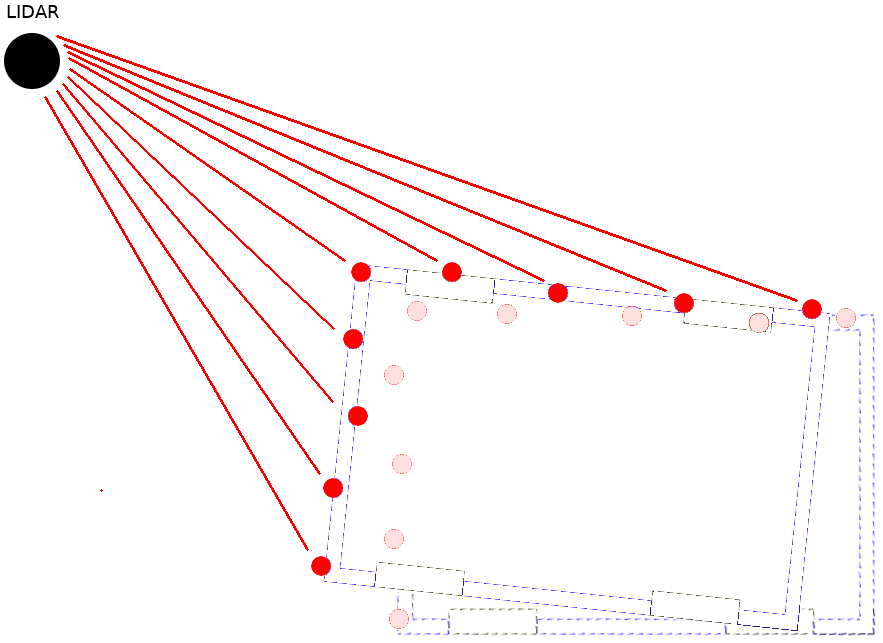
\includegraphics[height=80mm]{figures/raw/obstacle_movement_lidar.png}
    \caption{The detected points of the moving obstacle}
    \label{obstacle_movement_lidar}
\end{figure}

To understand the method of dynamic point detection, I removed the LIDAR, its virtual rays and the obstacle's contour from the image, thus leaving leaving only the measured points of the two timesnap. The result, which is basically a time-buffered array of 2D points, is presented on figure \ref{obstacle_movement_lidar_only}. The algorithm iterates through each point in the current measurement, and checks if any point in the previous measurements\footnote{The number of measurements to 'look up' is configurable.} is within its compliance radius\footnote{The compliance radius is a maximum allowed distance between measurements representing the same physical point but measured in different timesnaps. If the distance between two measurements is greater than this value, the measurements are assumed to represent different points of the space. The compliance radius is calculated for each measurement separately, and it is proportional to the distance of the LIDAR and the measured point.}.

\begin{figure}[!ht]
    \centering
    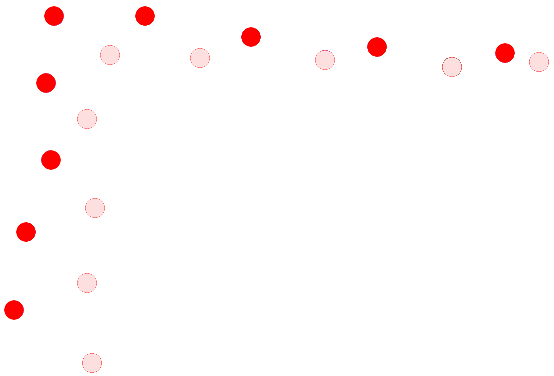
\includegraphics[height=50mm]{figures/raw/obstacle_movement_lidar_only.png}
    \caption{The detected points of the two timesnaps}
    \label{obstacle_movement_lidar_only}
\end{figure}

The measured points with their compliance radiuses are presented in \autoref{compliance_radiuses}. The possible dynamic points, that have no points from the previous measurement within their radius, are marked with blue, and their compliance radius with yellow. The possible static points are marked with red, along with their radiuses. Note, that these points are \textit{possible} dynamic and static points. The final classification will be preceded be multiple filtering mechanisms and point grouping, but this is the base for finding dynamic objects.

\begin{figure}[!ht]
    \centering
    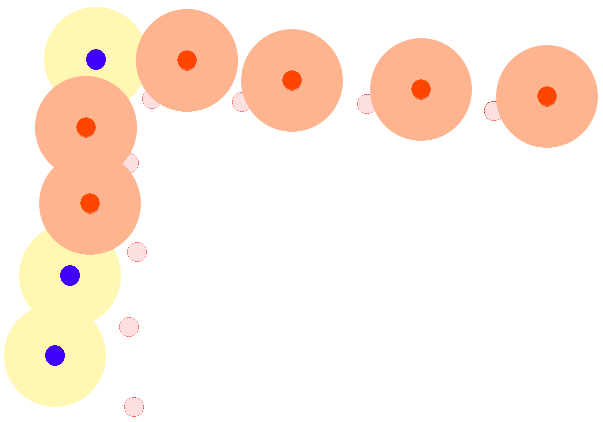
\includegraphics[height=50mm]{figures/raw/compliance_radiuses.png}
    \caption{The compliance radiuses and the dynamic points}
    \label{compliance_radiuses}
\end{figure}

Several conclusions can be drew from \autoref{compliance_radiuses}. The one, and probably most important is that with right parameterizing (number of 'look-up' measurements, compliance radius, etc) this method amplifies the positive\footnote{Previously a distant background was detected, but now a closer object appears.} and negative\footnote{Previously a close object was detected, but now it disappears, and the distant background becomes visible.} changes of the scans. The second remark is that the method does not detect all the points of a moving object. However, due to measurement noise, false detections may happen, and non-moving points may be marked as dynamic.

Therefore, the result of this separation step needs to be filtered. I implemented a filtering step that only keeps those samples in the set of dynamic points, of which the left and right neighbour in the scan has also been marked dynamic. It can be easily compared to \href{https://en.wikipedia.org/wiki/Erosion_(morphology)}{erosion} in image processing, which is able to remove peaks from the image. Let's take a look at \autoref{dynamic_points}. The possible dynamic points are marked with blue. The filtering mechanism iterates through each of them, and check both neighbours. As it can be easily read from the figure, point \textit{A} has two neighbours that have been marked static, therefore it will be removed from the set of dynamic points. However, points \textit{B} and \textit{C} both have dynamic neighbours (each other), so they will not be filtered out. This algorithm removes the single-size false detections from the result of the separation.

\begin{figure}[!ht]
    \centering
    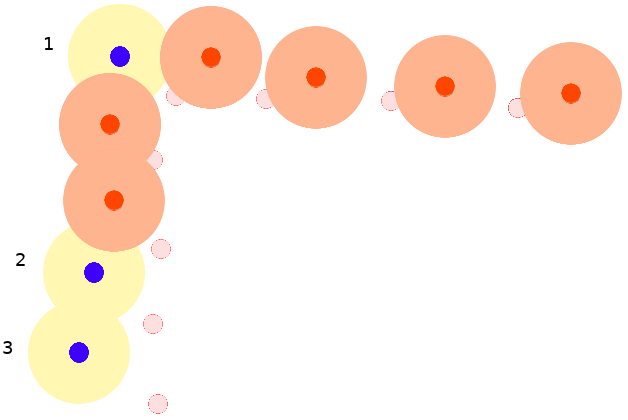
\includegraphics[height=50mm]{figures/raw/dynamic_points.png}
    \caption{Point \textit{A} will be filtered out}
    \label{dynamic_points}
\end{figure}

\subsection{Grouping}
After the filtering, we can safely assumed that the elements in the dynamic point set are in fact points of a moving obstacle. The next step is grouping the corresponding dynamic points, and also adding those points to these groups that were prevoiusly marked as static, but they are part of a moving group. For example in \autoref{dynamic_points}, after the separation and filtering, only points \textit{B} and \textit{C} were marked dynamic, but actually, all the points in the image are points of the same object, that is moving. The grouping algorithm needs to be able to add these other points to the group as well.

The grouping algorithm is based on the supposition that coherent points are close to each other, while the distance between points of separate objects is larger. With a few exceptions, this statement holds its stand, by practice it proved to be a reliable base for grouping. The algorithm itself is quite simple, it separates the list of measurements (including the static and dynamic poitns as well) into subsets - groups. A new group is started when the distance between two adjacent points is larger than the permitted maximum within a group. This maximum is an empirical constant, with experiments of valid use cases. The result of the step is shown in \autoref{groups}.

\begin{figure}[!ht]
    \centering
    \subfloat[Gazebo simulation]
    {
        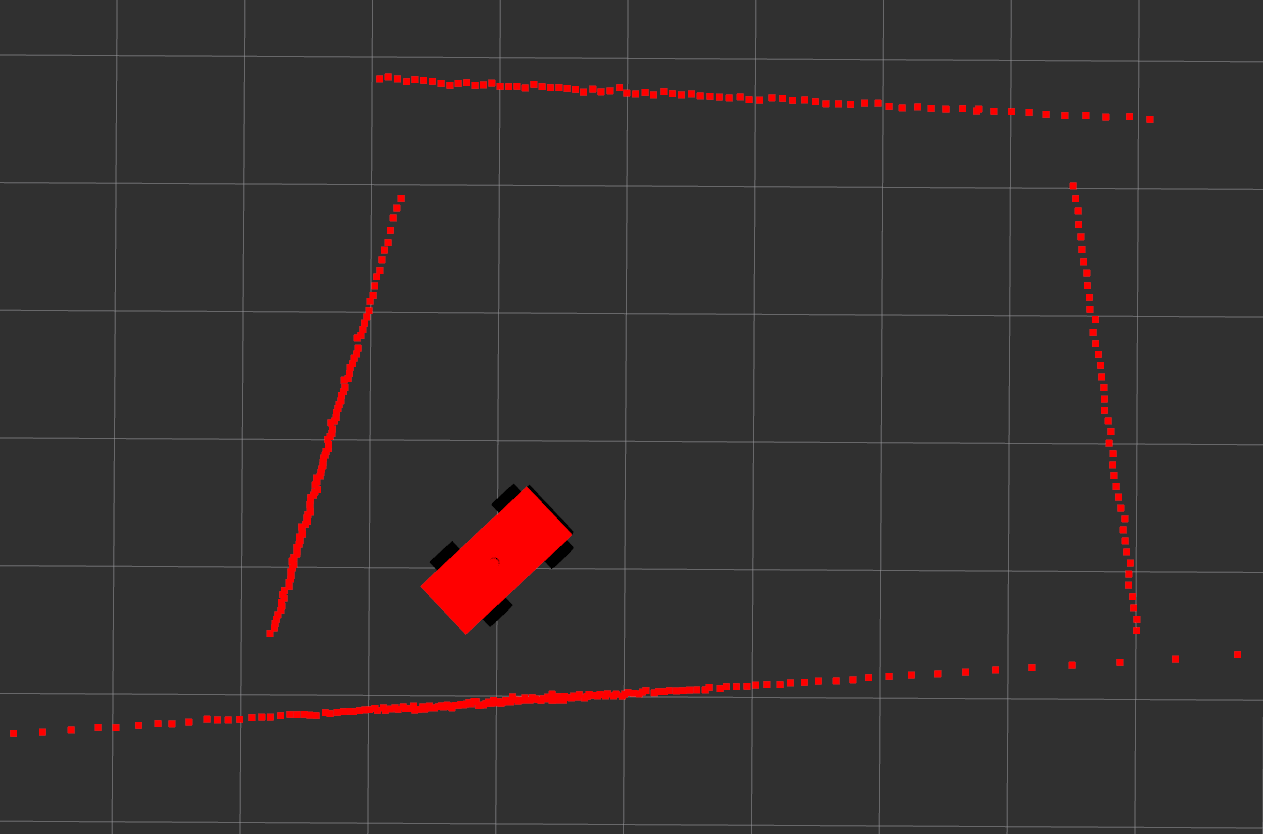
\includegraphics[height=46mm]{figures/raw/rviz_lidar_scan.png}
        \label{gazebo_wall_following_car}
    }
    \subfloat[Groups]
    {
    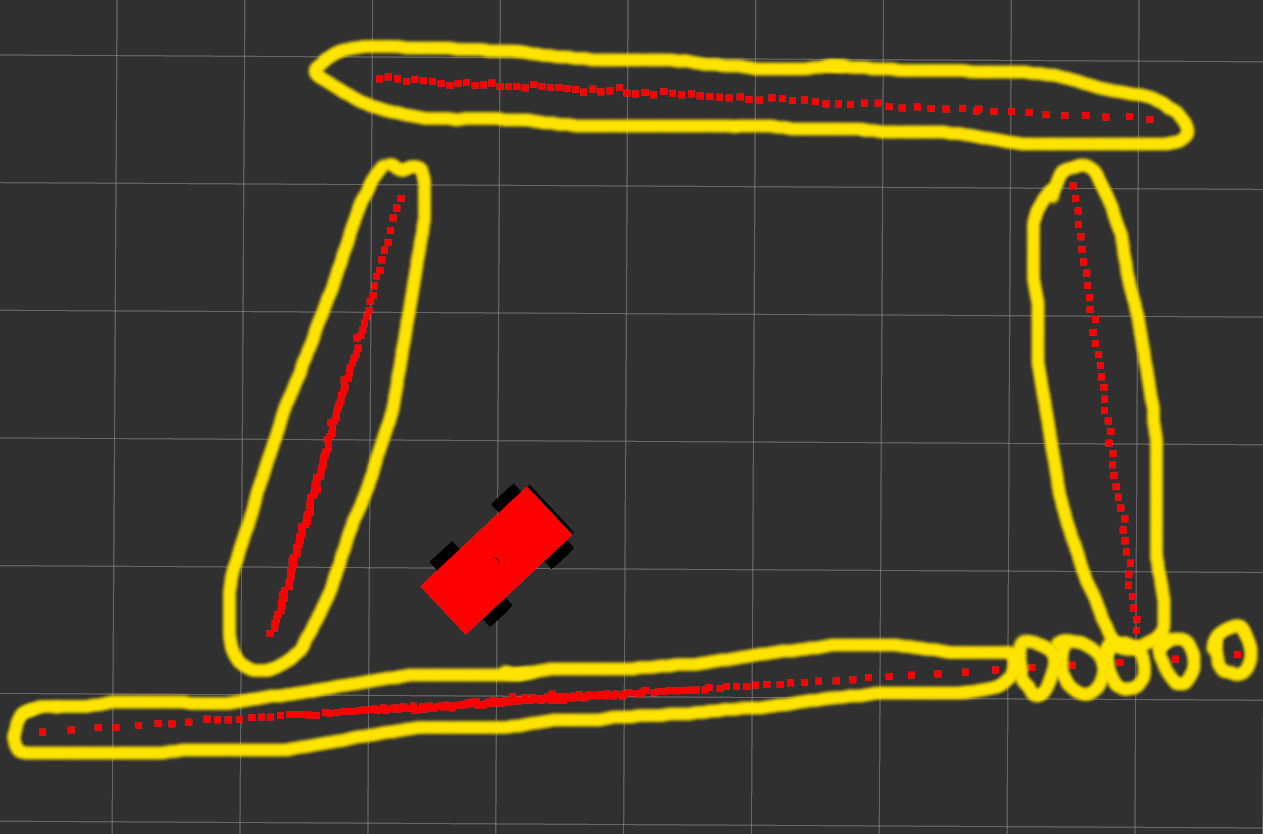
\includegraphics[height=46mm]{figures/raw/groups.png}
        \label{groups}
    }
    \caption{Distance-based grouping}
    \label{wall_following_car}
\end{figure}

As it is clearly visible on the image, far points that are correspondent to the same object may be separated from each other, and grouped one by one - see the bottom right corner of the picture. However, the further an object is from the LIDAR, the less important it is for the local trajectory planner, which needs to avoid close obstacles. But still, they are not valid groups, so as the last step of the grouping mechanism, these single-point groups will be removed from the list of groups. But before doing that, there is still one special case that needs to be handled by the grouping unit - the \textit{wall following car}. Let's imagine the situation represented in \autoref{wall_following_car}. The detected obstacle (represented by the box) is moving alongside the wall, and within the maximum group point distance. Therefore, the grouping algorithm will join the groups. This wouldn't be a problem if the box wasn't moving, but as soon as it changes its position, grouping it together with the wall would ruin the mass center and speed vector calculation, described in \autoref{chap:tracking}.

\begin{figure}[!ht]
    \centering
    \subfloat[Gazebo simulation]
    {
        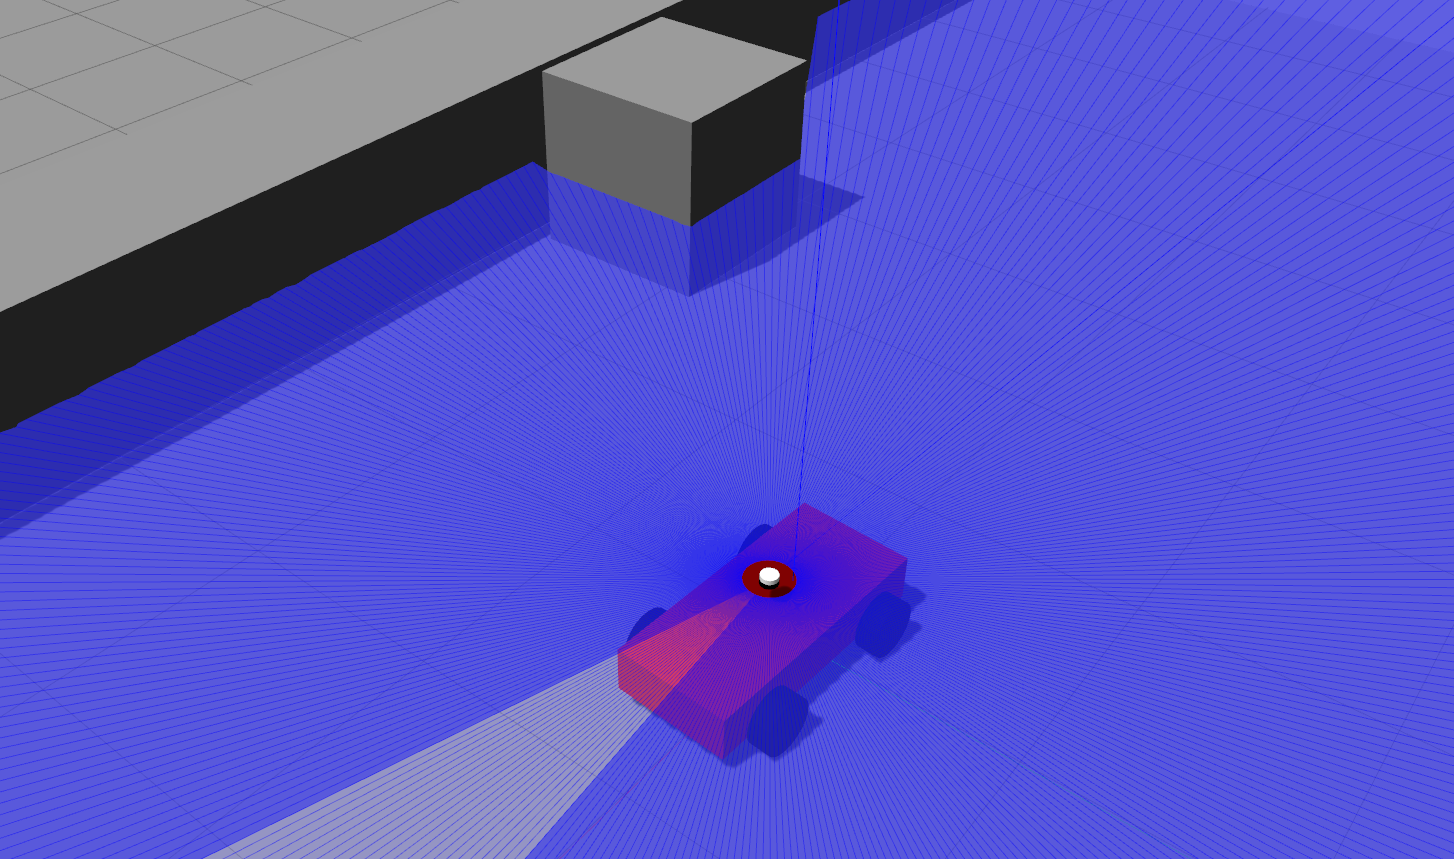
\includegraphics[height=46mm]{figures/raw/gazebo_wall_following_car.png}
        \label{gazebo_wall_following_car}
    }
    \subfloat[Lidar scan]
    {
    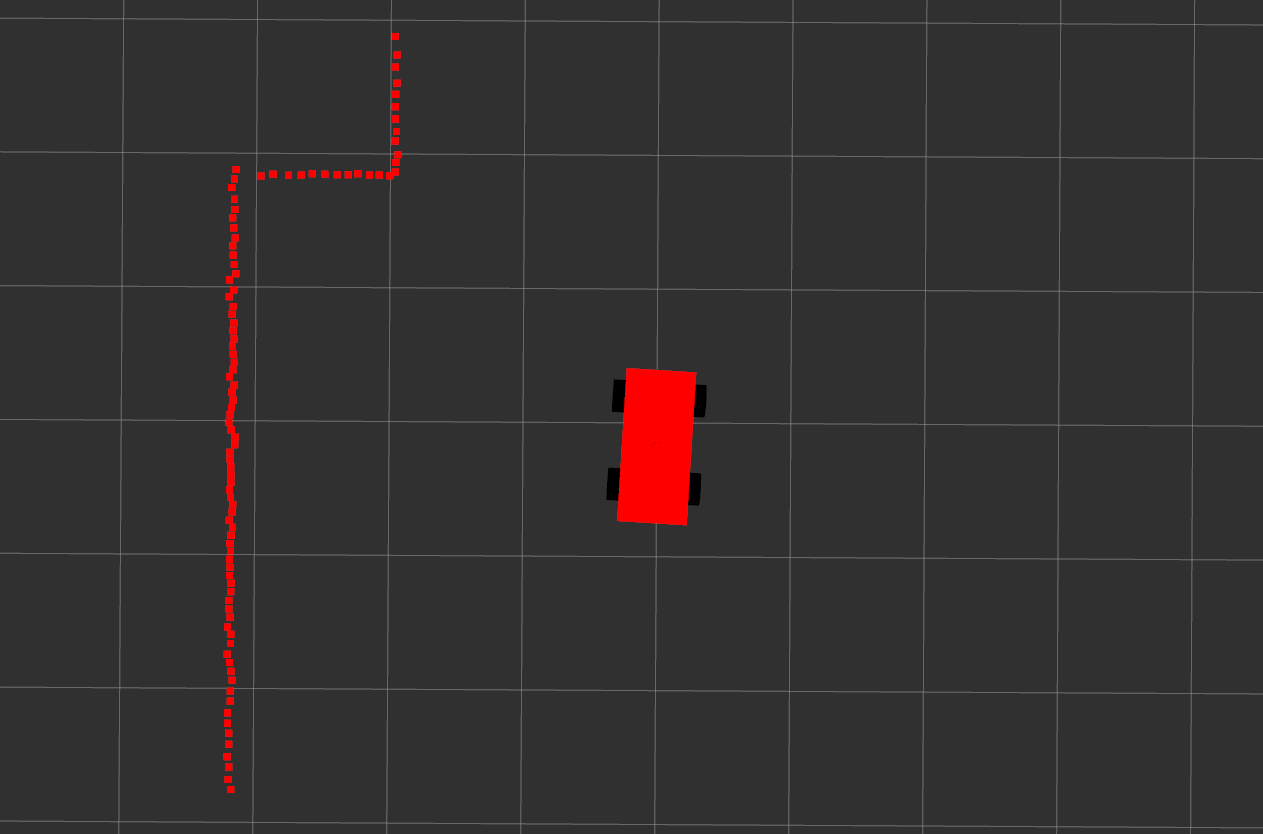
\includegraphics[height=46mm]{figures/raw/rviz_wall_following_car.png}
        \label{rviz_wall_following_car}
    }
    \caption{The \textit{wall following car}}
    \label{wall_following_car}
\end{figure}

To avoid this problem, the algorithm detects if an obstacle is unusually large, and cuts off long 'tails' from the group. Figure \autoref{group_cutting} explains this step in practice.

\begin{figure}[!ht]
    \centering
    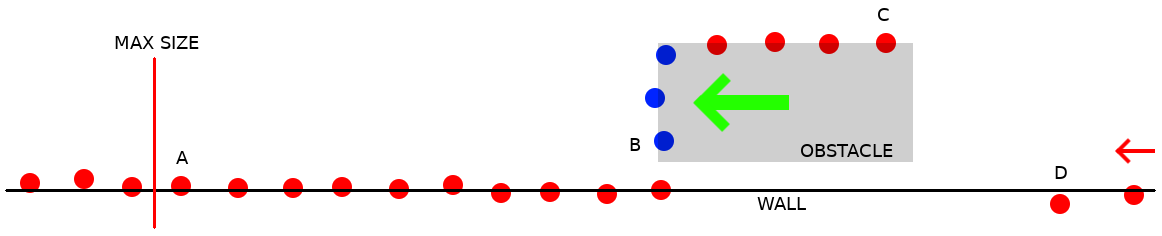
\includegraphics[width=\textwidth]{figures/raw/group_cutting.png}
    \caption{Points on the left of \textit{B} will be cut off}
    \label{group_cutting}
\end{figure}

Let's assume that the algorithm iterates through the points visualized in the figure from the right. The distance between points \textit{C} and \textit{D} is larger that the allowed maximum group point distance, therefore point \textit{C} starts a new group. Until the program reaches point \textit{A}, all the points are added to this group, because the distance between adjacent points is always lower than the maximum group point distance, but after point \textit{A}, the algorithm detects that the group is larger than the permitted limit. So the iteration turns around, and all the points are getting removed from the group, until the first dynamic point is reached - in the current example this would be point \textit{B}. As a result, only the points between (and including) point \textit{B} and point \textit{C} will be grouped together.

As an undesired side-effect, this step may also remove some of those points from the group that are in fact parts of the moving object but were marked as static, because the removal only stops at the first \textit{dynamic} point.

\subsection{Separation of static points and dynamic groups}

The previous step has successfully sorted the measured points into groups, but it is undecided yet if these groups are moving or not. This decision is made by checking the number of dynamic points in each group, which must exceed the required minimum in order to the group being marked as dynamic.

This was the last step of the separation of the groups, from this point, static points and dynamic groups will be handled differently.

\section{Dynamic obstacles}
After the dynamic groups have been separated from the static points, additional information needs to be calculated for them, so that the local track planner algorithm can use their data for its obstacle-avoidance feature. 3 pieces of information are needed for each object, its position, size and speed vector. All of these are calculated from the object's mass center, which is the average of the group points. This mass center is considered to be the object's position in space.

\begin{figure}[!ht]
    \centering
    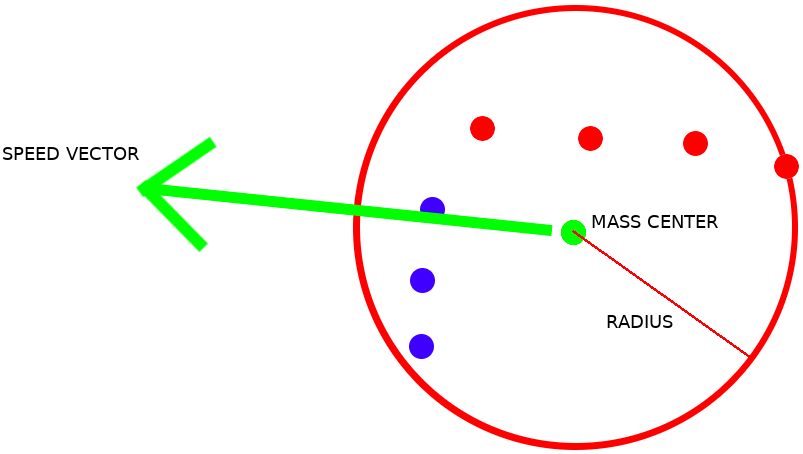
\includegraphics[height=50mm]{figures/raw/dynamic_information.png}
    \caption{The calculated information for dynamic obstacles}
    \label{dynamic_information}
\end{figure}

\subsection{Areas}
First, the groups are substituted by bounding circles. The circle's radius is the distance between the farthest group point and the mass center. This simplification results in easier path calculation in the local planner, but also drops every information known about the obstacle's shape. For long objects, for instance, this method provides a very unrealistic image of the object, because the bounding circle is much larger than the obstacle itself. But for ususal shapes such as cars, the loss that the representation causes is less than the processing time we save with the simplification.

\subsection{Tracking}
\label{chap:tracking}
Speed vectors are calculated from the change of the mass center between measurements. But in order to be able to check the mass center of a group in any previous measurement, object tracking is needed. The tracking is done by estimating each obstacles' current position based on their previous positions and speed vectors, and finding the best fit among the current groups. Filtering is also needed for such false detections when a previously detected object is not recognized for a few cycles. Without filtering, these obstacles would disappear from the list of groups for a period of time and then they would reappear, but tracking would fail. Therefore the algorithm keeps these objects alive for a given number of measurement periods, updating their positions with their last known speed vector in every cycle.

\begin{figure}[!ht]
    \centering
    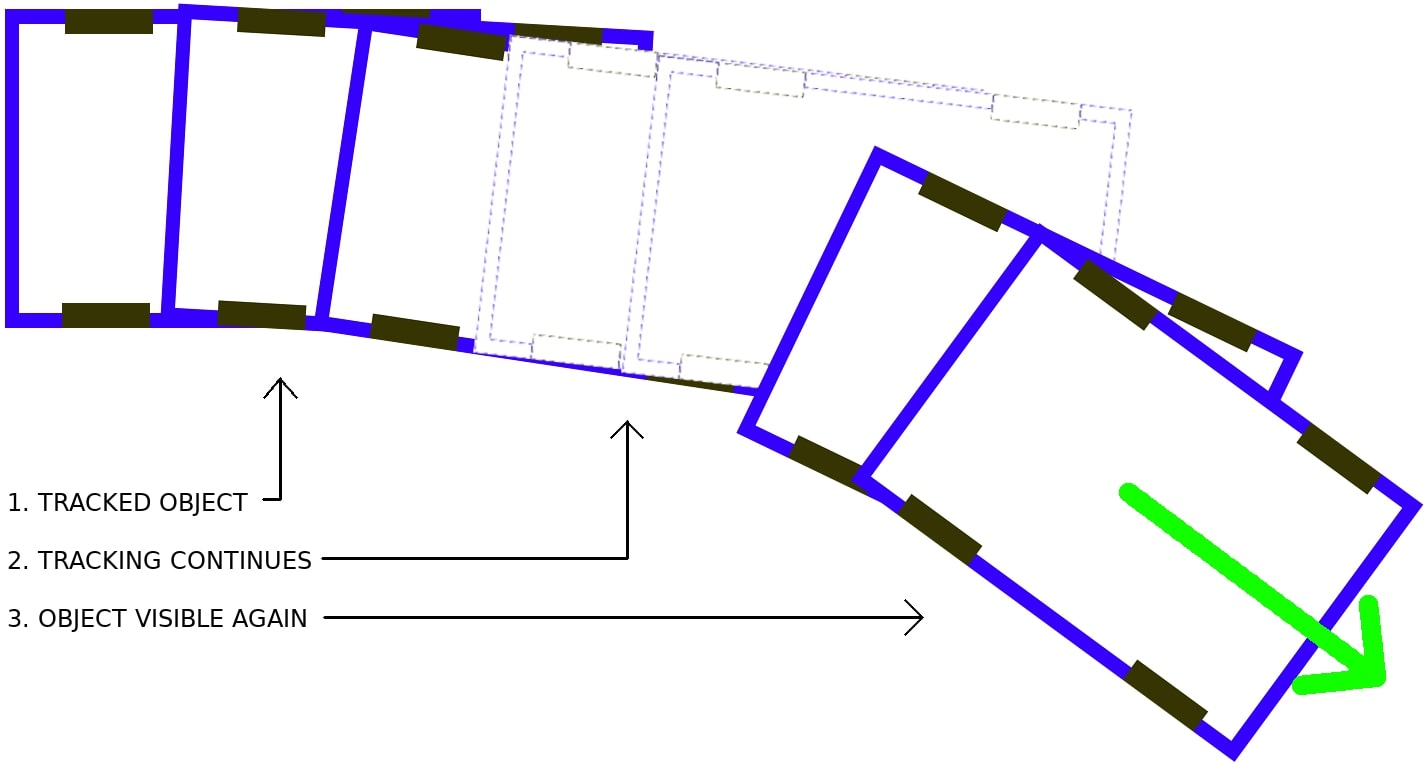
\includegraphics[width=\textwidth]{figures/raw/tracking.png}
    \caption{Object tracking}
    \label{tracking}
\end{figure}

After the objects have been tracked, their speed vectors can be calculated. A filter is applied here, as well, for smoother obstacle paths.

\subsection{Publishing dynamic obstacles}
Dynamic obstacles - as outputs of the mapping node - are published on several topics, responsible for containing information for either further processing or visualization. The standard dynamic object structure in which moving objects are published to the local planner is not defined yet. The visualization messages, however, are implemented and in active use.

\begin{figure}[!ht]
    \centering
    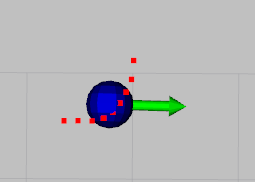
\includegraphics[height=50mm]{figures/raw/rviz_moving_object.png}
    \caption{Visualizing moving objects}
    \label{rviz_moving_object}
\end{figure}

The published messages contain \textit{visualization\_msgs::Marker} instances with either \textit{SPHERE} or \textit{ARROW} instances with either \textit{SPHERE} or \textit{ARROW} type, thus representing the areas and speed vectors of the objects.

\section{Static points}
Static points used for two separate purposes. The first one is building a static map, the second is localization with the help of gmapping.

\subsection{Static map}
\label{chap:static_map}
After separating the dynamic groups from the scan points, only the static points are left. These points do not change their positions with time\footnote{Except those obstacles that start moving only after they have already been detected as sets of static points. But these objects do not ruin the quality of the map, either.}, so they can be added to the static map.

For static map-building, gmapping has already been mentioned as a candidate, but unfortunately, its algorithm does not recognize changes in the environment. In practice, if an object has been detected and placed in its map, it will not be erased from there, even after the object has moved away. Figures \ref{gmapping_drawback_before_move} and \ref{gmapping_drawback_after_move} demonstrate the problem.

\begin{figure}[!ht]
    \centering
    \subfloat[Gazebo simulation]
    {
        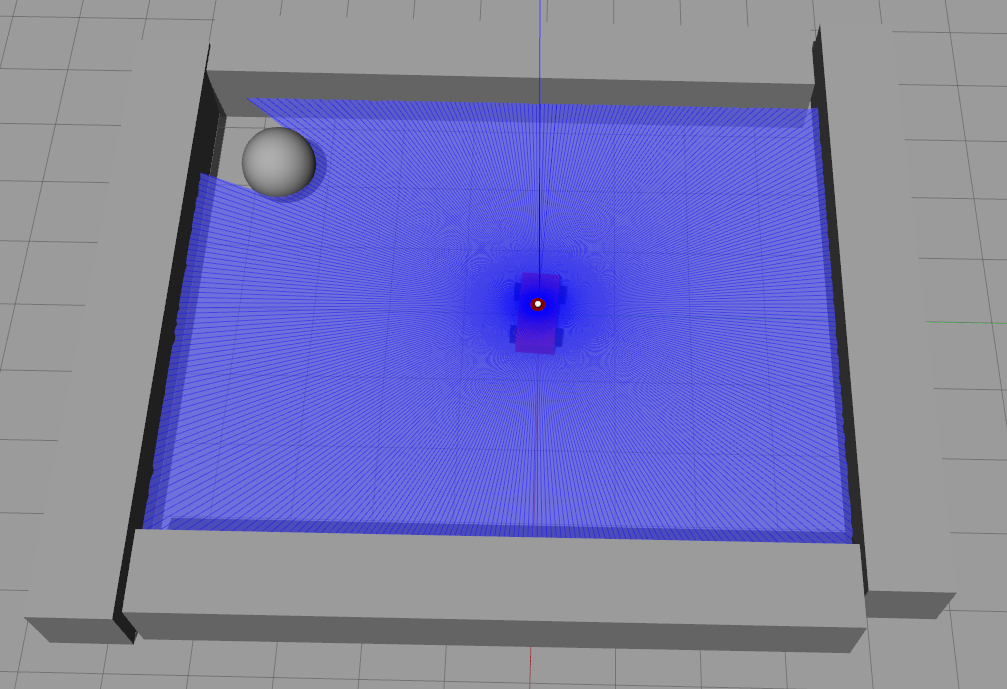
\includegraphics[height=48mm]{figures/raw/gazebo_gmapping_before_move.png}
        \label{gazebo_gmapping_before_move}
    }
    \subfloat[Map created by gmapping]
    {
    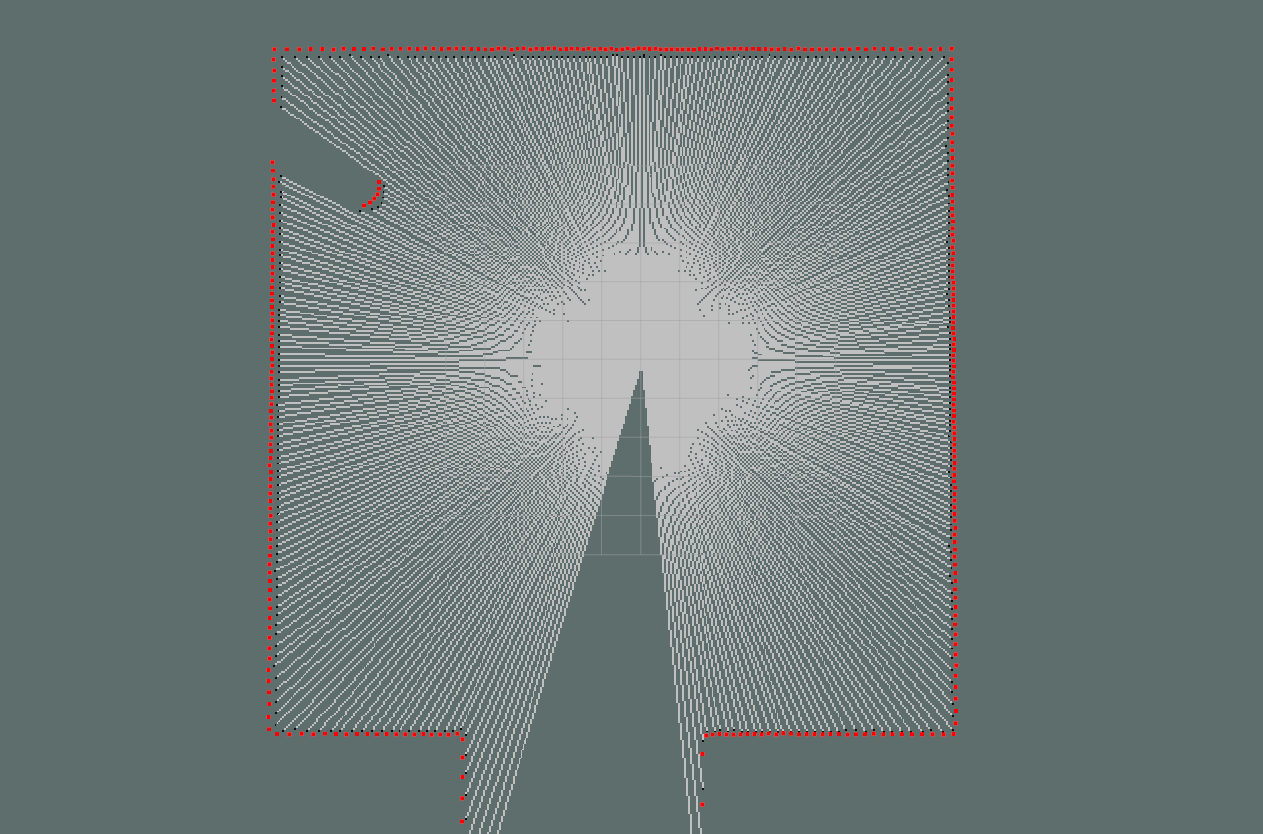
\includegraphics[height=48mm]{figures/raw/rviz_gmapping_before_move.png}
        \label{rviz_gmapping_before_move}
    }
    \caption{Initial state - ball is still}
    \label{gmapping_drawback_before_move}
\end{figure}

\autoref{gmapping_drawback_before_move} shows a situation where the ball is standing still. The mapping algorithm of gmapping successfully creates a map (in the form of an occupancy grid\footnote{An occupancy grid represents a map in an evenly spaced field of probability values representing if the grid points are occupied by an obstacle}) that marks the place of the ball as occupied. However, when the ball starts moving (see \autoref{gmapping_drawback_after_move}), the map does not change, because the algorithm cannot handle moving obstacles.

\begin{figure}[!ht]
    \centering
    \subfloat[Gazebo simulation]
    {
        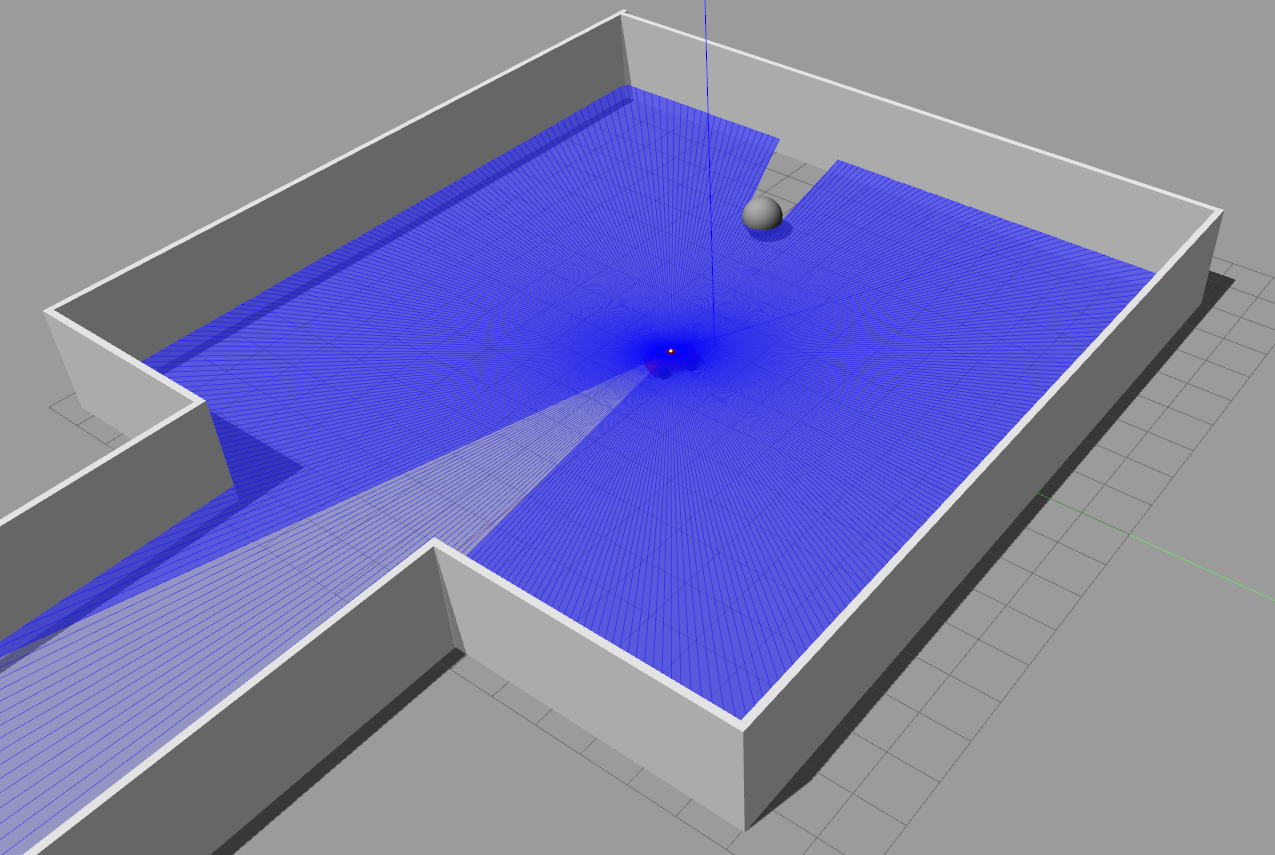
\includegraphics[height=48mm]{figures/raw/gazebo_gmapping_after_move.png}
        \label{gazebo_gmapping_after_move}
    }
    \subfloat[Map created by gmapping]
    {
        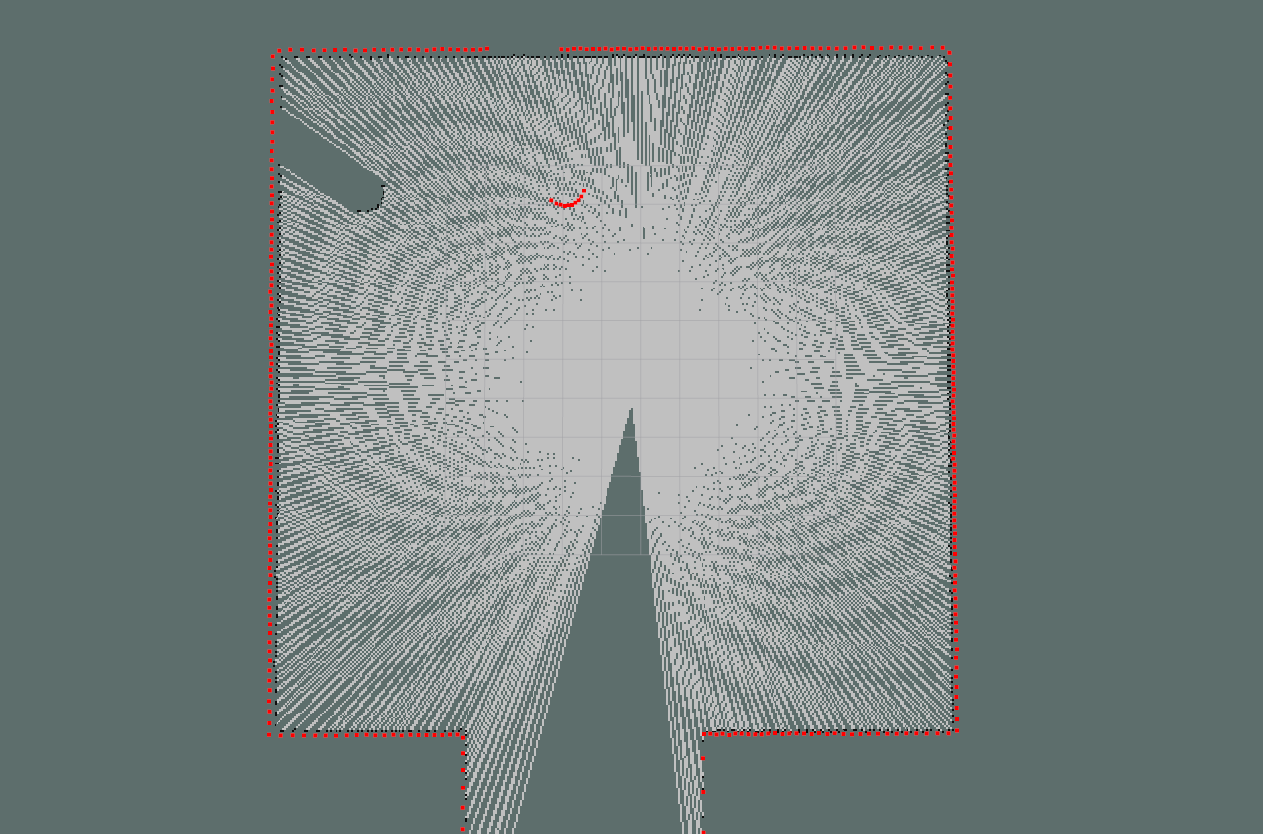
\includegraphics[height=48mm]{figures/raw/rviz_gmapping_after_move.png}
        \label{rviz_gmapping_after_move}
    }
    \caption{Moving state - ball has changed position}
    \label{gmapping_drawback_after_move}
\end{figure}

Due to the above problem, static map-building needed to be implemented internally, which is basically a 2D occupancy grid. The grid points' possible values are the following:

\begin{center}
    \begin{tabular}{ c c }
        
\includegraphics[height=3mm]{figures/raw/map_occupied.png} & Occupied (value: 100) \\
        
\includegraphics[height=3mm]{figures/raw/map_unknown.png}  & Unknown (value: 50)   \\
        
\includegraphics[height=3mm]{figures/raw/map_free.png}     & Free (value: 0)       \\
    \end{tabular}
\end{center}

I chose the most straight-forward way of map-building - each static measurement introduces an occupied point and a free ray in the map. \autoref{map_ray} visualizes the situation. The green and red grids are the car's current position and the measured point.

\begin{figure}[!ht]
    \centering
    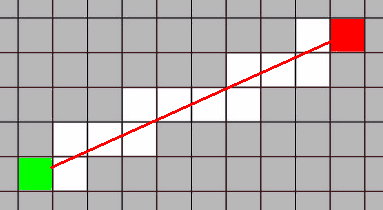
\includegraphics[height=50mm]{figures/raw/map_ray.png}
    \caption{Introducing a free ray}
    \label{map_ray}
\end{figure}

\subsection{Publishing static scan}
As I mentioned already, gmapping is not used as a primary map-builder node, but its localization is still useful, therefore LIDAR measurements still need to be published for it. As the algorithm already separated the static points from the dynamic ones, it is handy to publish only the static measurements to gmapping. So in this step, a new scan structure is created, but the dynamic points are not added to it, only the static ones.

\section{Conclusion}
As a conclusion of the mapping sub-project, I present an example with a valid use-case. The scenario is the following. The car is standing in a closed room, the distance from the walls are smaller than the LIDAR's range. There is one other object in the room, in the simulation, this is a ball, its size similar to the car's. The ball is standing in one place at first, but after a while, it start moving in a straight path with constant speed. Finally, the car starts moving as well - first in a straight path, then turning.

\autoref{mapping_demo_start} presents the initial situation of the demonstration. The left image shows the simulation - the car is standing in the middle of the room, the object in the top left corner is not moving yet. On the right image, the created static map is visible. The number of unknown (grey) grid points is large at this state of the simulation, it will dramatically decrease once the car starts moving. This effect is caused by the LIDAR's finite angular resolution and ray characteristics. The black grid points represent statically occupied positions. All the walls are marked static, and the ball as well.

\begin{figure}[!ht]
    \centering
    \subfloat[Gazebo simulation]
    {
        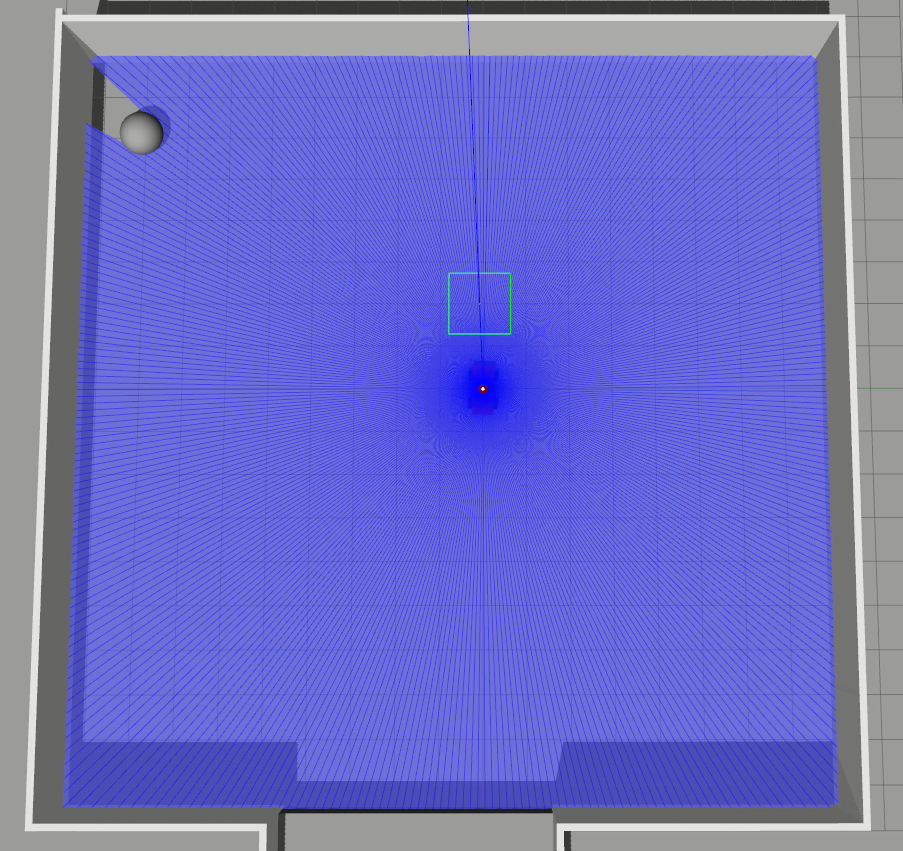
\includegraphics[height=70mm]{figures/raw/mapping_demo/gazebo_start.png}
        \label{mapping_demo_gazebo_start}
    }
    \subfloat[rviz visualization]
    {
    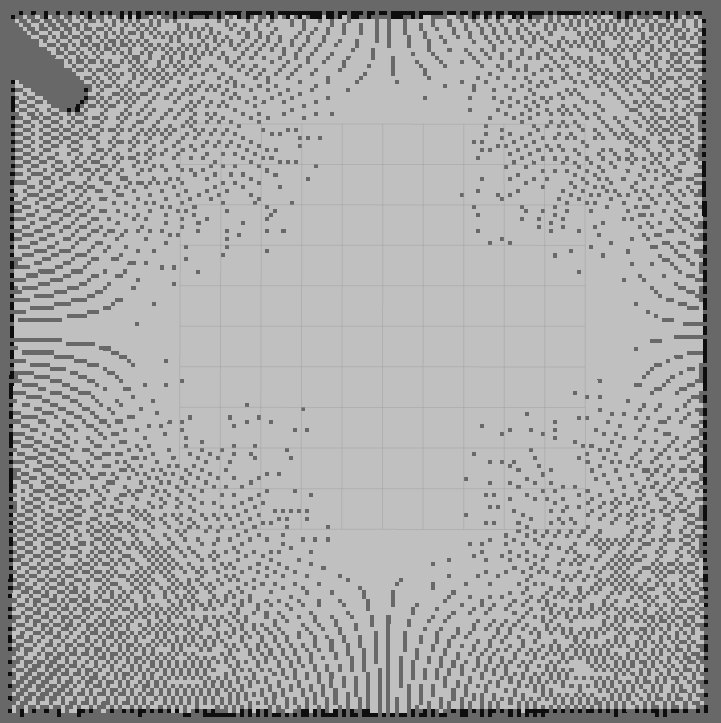
\includegraphics[height=70mm]{figures/raw/mapping_demo/rviz_start.png}
        \label{mapping_demo_rviz_start}
    }
    \caption{Initial state - ball is still}
    \label{mapping_demo_start}
\end{figure}

Once the ball starts moving (\autoref{mapping_demo_ball_moving}), it stops being marked as static, but is handled as a moving object. The static block at the top left corner has been removed, and the ball is displayed using the dynamic visualization toolset - a sphere and an arrow, representing the ball's area and speed vector.

\begin{figure}[!ht]
    \centering
    \subfloat[Gazebo simulation]
    {
        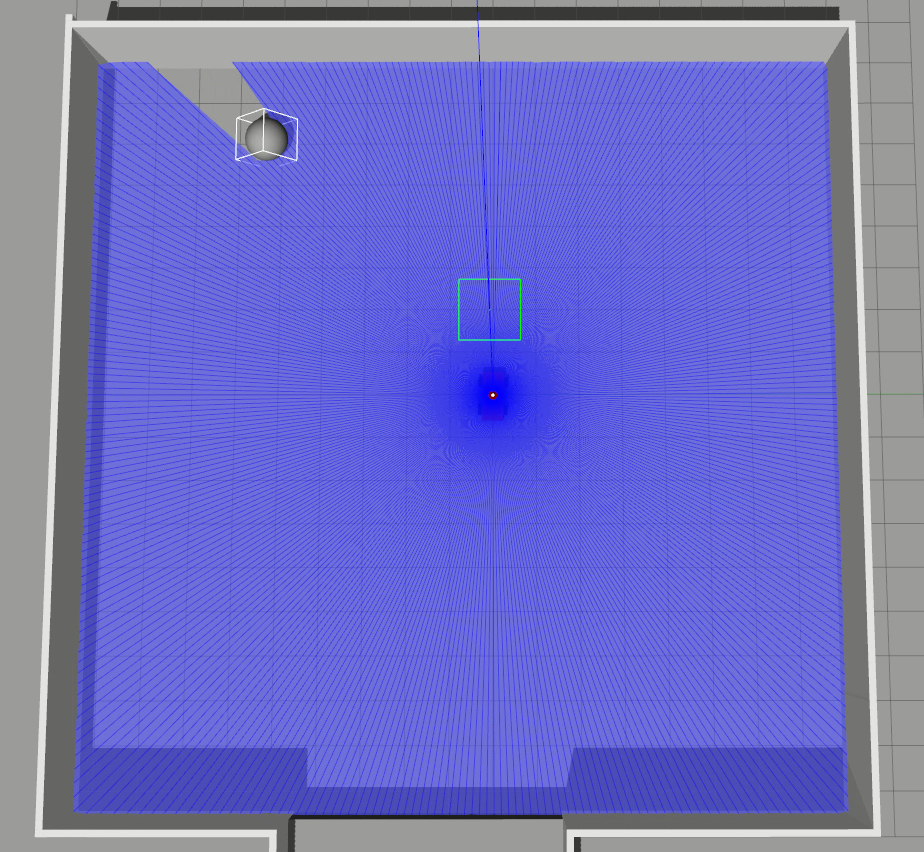
\includegraphics[height=70mm]{figures/raw/mapping_demo/gazebo_ball_moving.png}
        \label{mapping_demo_gazebo_ball_moving}
    }
    \subfloat[rviz visualization]
    {
    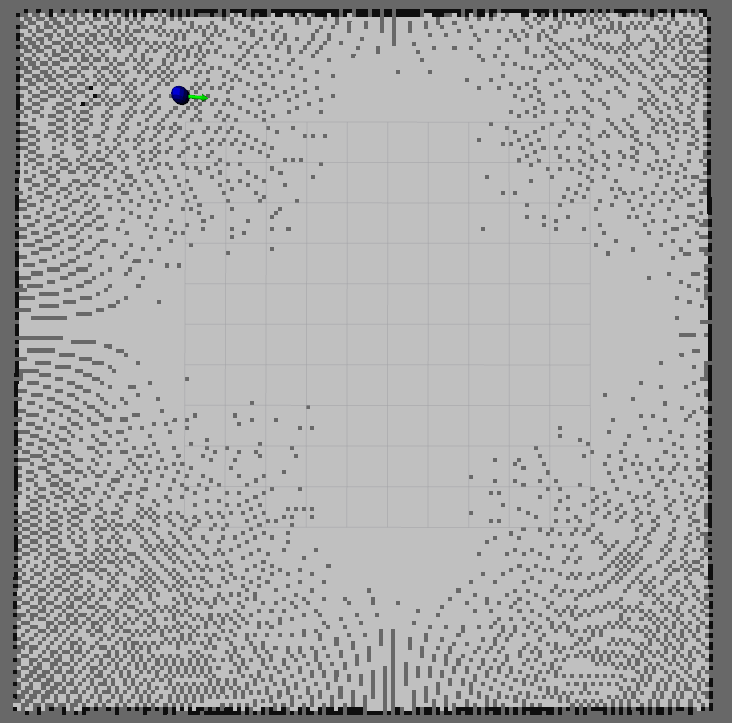
\includegraphics[height=70mm]{figures/raw/mapping_demo/rviz_ball_moving.png}
        \label{mapping_demo_rviz_ball_moving}
    }
    \caption{The ball is moving}
    \label{mapping_demo_ball_moving}
\end{figure}

When the car starts moving, the map immediately starts to clear out. If we compare \autoref{mapping_demo_ball_moving} and \autoref{mapping_demo_car_moving}, it is clear that the latter contains less unknown grid points. The dynamic object-tracking is still operating without error, the ball's speed vector is correct.

\begin{figure}[!ht]
    \centering
    \subfloat[Gazebo simulation]
    {
        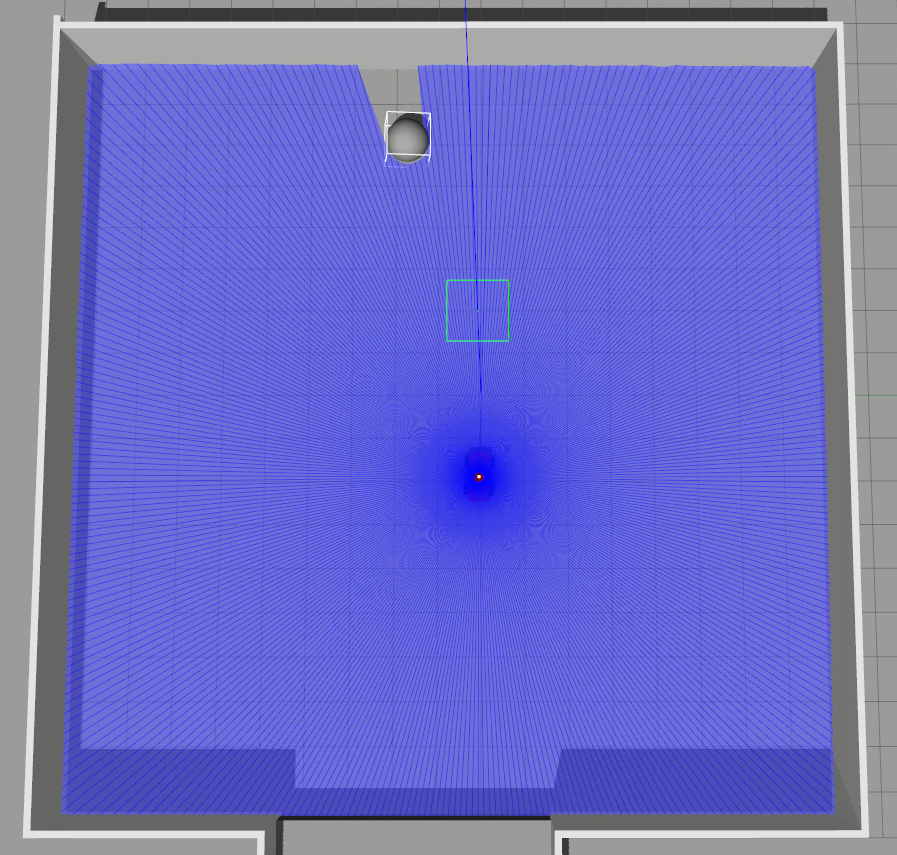
\includegraphics[height=70mm]{figures/raw/mapping_demo/gazebo_car_moving.png}
        \label{mapping_demo_gazebo_car_moving}
    }
    \subfloat[rviz visualization]
    {
    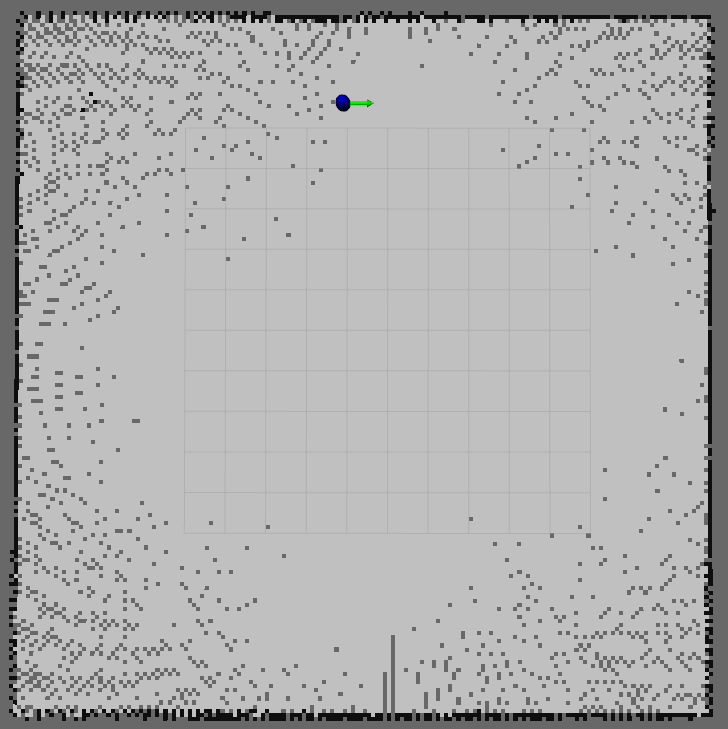
\includegraphics[height=70mm]{figures/raw/mapping_demo/rviz_car_moving.png}
        \label{mapping_demo_rviz_car_moving}
    }
    \caption{The car is moving}
    \label{mapping_demo_car_moving}
\end{figure}

However, as soon as the car starts turning instead of moving in a straight trajectory, the measurements become very noisy. \autoref{mapping_demo_car_turning} demonstrates the situation. The simulation image (left) shows that the LIDAR scan has a rotational error. Reflecting to this noise, the static-dynamic separation and tracking do not work properly, the algorithm keeps losing objects and then finding them again. It is also visible on the right-hand image, that the rotational error has undesired effects in the static map. The walls are duplicated and are not necessarily at their correct position.

\begin{figure}[!ht]
    \centering
    \subfloat[Gazebo simulation]
    {
        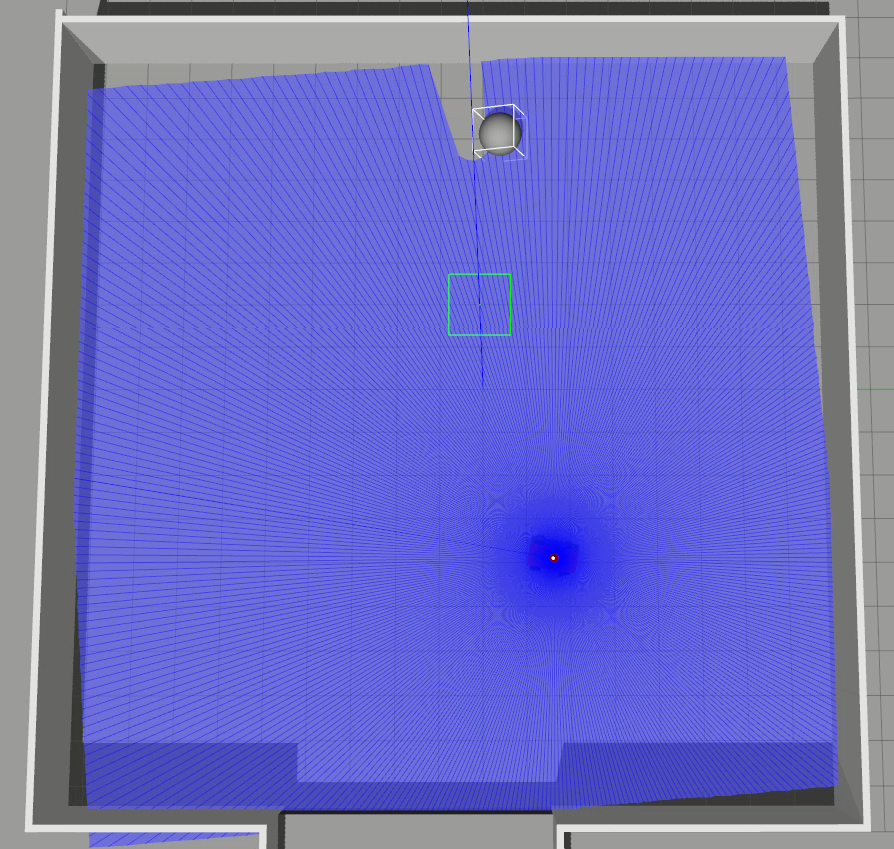
\includegraphics[height=70mm]{figures/raw/mapping_demo/gazebo_car_turning.png}
        \label{mapping_demo_gazebo_car_turning}
    }
    \subfloat[rviz visualization]
    {
    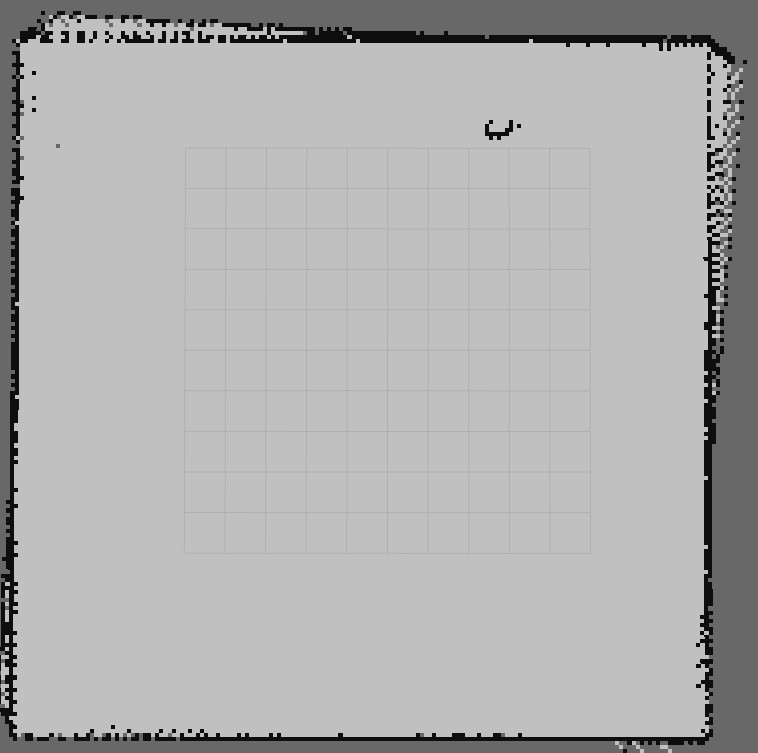
\includegraphics[height=70mm]{figures/raw/mapping_demo/rviz_car_turning.png}
        \label{mapping_demo_rviz_car_turning}
    }
    \caption{The car is turning}
    \label{mapping_demo_car_turning}
\end{figure}

Due to the above mentioned problems, the mapping node can only be used with certain limitations regarding obstacle speed and the car's angular velocity. These problems will be solved in the future, using more leniant filtering for existing dynamic groups and a more advanced static mapping algorithm.
\include{content/planning}
\include{content/summary}

% Acknowledgements
%~~~~~~~~~~~~~~~~~~~~~~~~~~~~~~~~~~~~~~~~~~~~~~~~~~~~~~~~~~~~~~~~~~~~~~~~~~~~~~~~~~~~~~
%\chapter*{Acknowledgments}

The research presented in this thesis work has been carried out in the frame of project no. FIEK\_16-1-2016-0007, which has been implemented with the support provided from the National Research, Development and Innovation Fund of Hungary, financed under the Center for Higher Education and Industrial Cooperation - Research infrastructure development (FIEK\_16) funding scheme.


% List of Figures, Tables
%~~~~~~~~~~~~~~~~~~~~~~~~~~~~~~~~~~~~~~~~~~~~~~~~~~~~~~~~~~~~~~~~~~~~~~~~~~~~~~~~~~~~~~
%\listoffigures\addcontentsline{toc}{chapter}{\listfigurename}
%\listoftables\addcontentsline{toc}{chapter}{\listtablename}


% Bibliography
%~~~~~~~~~~~~~~~~~~~~~~~~~~~~~~~~~~~~~~~~~~~~~~~~~~~~~~~~~~~~~~~~~~~~~~~~~~~~~~~~~~~~~~
\addcontentsline{toc}{chapter}{\bibname}
\bibliography{bib/mybib}


% Appendix
%~~~~~~~~~~~~~~~~~~~~~~~~~~~~~~~~~~~~~~~~~~~~~~~~~~~~~~~~~~~~~~~~~~~~~~~~~~~~~~~~~~~~~~
%%----------------------------------------------------------------------------
\appendix
%----------------------------------------------------------------------------
\chapter*{\fuggelek}\addcontentsline{toc}{chapter}{\fuggelek}
\setcounter{chapter}{\appendixnumber}
%\setcounter{equation}{0} % a fofejezet-szamlalo az angol ABC 6. betuje (F) lesz
\numberwithin{equation}{section}
\numberwithin{figure}{section}
\numberwithin{lstlisting}{section}
%\numberwithin{tabular}{section}

%\label{page:last}
\end{document}
